%\documentclass{jss}
\documentclass[nojss]{jss}
\usepackage[OT1]{fontenc}
\usepackage{amsmath,lifecon,thumbpdf}
%\usepackage{myVignette}
%\VignetteIndexEntry{An introduction to lifecontingencies package}
%\VignetteKeywords{vig1}
%\VignettePackage{lifecontingencies}
% need no \usepackage{Sweave.sty}
%\SweaveOpts{prefix.string=Figures/fig}
\author{Giorgio Alfredo Spedicato\\StatisticalAdvisor}
\Plainauthor{Giorgio Alfredo Spedicato}

\title{The \pkg{lifecontingencies} Package: Performing Financial and Actuarial Mathematics Calculations in \proglang{R}}
\Plaintitle{The lifecontingencies Package: Performing Financial and Actuarial Mathematics Calculations in R}
\Shorttitle{\pkg{lifecontingencies}: Financial and Actuarial Mathematics Calculations in \proglang{R}}

\Abstract{
  It is possible to model life contingency insurances with the
  \pkg{lifecontingencies} \proglang{R} package, which is capable of
  performing financial and actuarial mathematics calculations.  Its
  functions permit one to determine both the expected value and the
  stochastic distribution of insured benefits. Therefore, life
  insurance coverage can be priced and portfolios risk-based capital
  requirements can be assessed. This paper briefly summarizes the
  theory regarding life contingencies that is based on financial
  mathematics and demographic concepts. Then, with the aid of applied
  examples, it shows how the \pkg{lifecontingencies} package can be a
  useful tool for executing routine, deterministic, or stochastic
  calculations for life-contingencies actuarial mathematics.
}


\Keywords{life tables, financial mathematics, actuarial mathematics, life insurance}
\Plainkeywords{life tables, financial mathematics, actuarial mathematics, life insurance} %% without formatting
%% at least one keyword must be supplied

\Volume{55}
\Issue{10}
\Month{November}
\Year{2013}
\Submitdate{2012-04-10}
\Acceptdate{2013-04-03}

%% The address of (at least) one author should be given
%% in the following format:
\Address{
  Giorgio Alfredo Spedicato\\
  StatisticalAdvisor\\
  Via Firenze 11
  20037 Italy\\
  Telephone: +39/334/6634384\\
  E-mail: \email{lifecontingencies@statisticaladvisor.com}\\
  URL: \url{www.statisticaladvisor.com}
}



%% for those who use Sweave please include the following line (with % symbols):
%% need no \usepackage{Sweave.sty}

%% end of declarations %%%%%%%%%%%%%%%%%%%%%%%%%%%%%%%%%%%%%%%%%%%%%%%

\begin{document}


\maketitle

\section{Introduction}
This vignette is based on the package's paper published in JSS,
\cite{spedLifecon}. Apart of keeping track of package's updates, a major
difference with respect to JSS publication is that parallel features are turned
off to cope with CRAN packages' submission policies. As of March 2014, the
\pkg{lifecontingencies} package
\citep{spedLifecon} appears as the first \proglang{R} package that deals with life contingent actuarial mathematics. The \proglang{R}
statistical programming environment \citep{rSoftware} has become the
primary reference software for academics. Even in a business context,
\proglang{R} is now considered a valid alternative to affirmed
proprietary packages for statistics and data analysis, namely
\proglang{SAS} \citep{SAS}, \proglang{MATLAB} \citep{MATLAB} and
\proglang{SPSS} \citep{SPSS}. Some packages for actuarial applications
have already been developed within \proglang{R}. However, most of them
mainly focus on non-life insurance. In fact, non-life insurance
modeling involves more data analysis and applied statistical modeling
than that of life insurance. Functions allowing one to fit loss
distributions and perform credibility analysis are provided within the
package \pkg{actuar} \citep{Dutang2008}. This package represents the
computational side of the classical actuarial textbook on loss
distribution \citep{klugman2009loss}. The package \pkg{ChainLadder}
\citep{chainLadder} provides functions that are capable of estimating
loss reserves for non-life insurance. Generalized linear models
(GLMs), widely used in non-life insurance rate-making, can be fit by
functions bundled within base \proglang{R} distributions. The
generalized additive models for location, shape and scale (GAMLSS) and
tweedie regression, which are both more advanced predictive models
used by actuaries, are handled by specifically developed packages such
as \pkg{gamlss} \citep{gamlssPkg,gamlsspkg2} and \pkg{cplm} \citep{cplmPkg}.

Life insurance actuarial work deals mainly with demographic and
financial data.  The CRAN task view ``Empirical Finance''
\citep{taskview} lists several packages tailored specifically for
financial analysis. Packages \pkg{YieldCurve} \citep{YieldCurveR} and
\pkg{termstrc} \citep{termstrcR} are capable of financial modeling for
interest rates. Among the few packages that handle demographic data,
\pkg{demography} \citep{demographyR} and \pkg{LifeTables}
\citep{LifeTableR} can be used to manage demographic projections and
life tables.

On the other hand, many commercial software packages tailored
specifically for the actuarial analysis of life insurance are already
available. \pkg{MoSes} \citep{moses} and \pkg{Prophet}
\citep{prophet} are currently the leading actuarial software packages
for life insurance modeling. The \pkg{lifecontingencies} package aims
to represent the computational \proglang{R} companion of the
theoretical concepts exposed in textbooks like the classical
\cite{bowers1997actuarial} and \cite{dickson2009actuarial} for
actuarial mathematics and \cite{broverman2008mathematics} for
financial mathematics. Package \pkg{lifecontingencies} is available from
the Comprehensive \proglang{R} Archive Network at
\url{http://CRAN.R-project.org/package=lifecontingencies}. The examples used throughout this
paper have been taken from \cite{mathFinAct} and \cite{finanMLC}, both
freely available financial and actuarial mathematics textbooks. The
paper is structured as follows: Section~\ref{sec:statistics} outlines
the statistical and financial mathematical theory regarding life
contingencies, Section~\ref{sec:structure} overviews the structure of
the \pkg{lifecontingencies} package, Section~\ref{sec:examples} gives
a wide choice of applied \pkg{lifecontingencies} examples, and
finally, Section~\ref{sec:discussion} discusses the packages current
and future development as well as its known limitations.


\section[Statistical and financial foundations of life
  contingencies]{Statistical and financial foundations of life
  contingencies}\label{sec:statistics}

The actuarial pricing and reserving of life contingent insurances
involves the calculation of statistics regarding occurrences and
amounts of future cash flows. For example, the insurance pure premium
(also known as benefit premium) can be regarded as the expected value
of the prospective benefits cash flow distribution, valued at time zero
for a given interest rate structure. The probabilities of the
prospective benefits cash flow are based on the occurrence of the
policyholder's life events (life contingencies). In addition, the
theory of interest is used to find the present value of these amounts
that will occur in the future. Therefore, life insurance actuarial
mathematics is based on concepts derived from demography and theory of
interest.

A life table (also called a mortality table or actuarial table) is a
table that shows how mortality affects subjects of a cohort across
different ages. For each age $x$, it reports the number of $l_x$
individuals living at the beginning of age $x$. It is a sequence of
$l_0, l_1, \ldots, l_{\omega}$, where $l_{\omega}$, the terminal age,
represents the latest age that a subject of the cohort can survive
until. Life tables are typically distinguished according to gender,
year of birth and nationality, with different categories being used
depending on the type of life contingency (i.e., assurance or
annuity). As another example, businesses may have different customers
with different underlying mortalities, so they will be in need of
different life tables.

From a statistical point of view, a life table allows one to deduce
the probability distribution of the future lifetime for a policyholder
aged $x$. In particular, a life table also permits one to derive two
key probability distributions: $\tilde T_x$, the complete future
lifetime for a policyholder aged $x$, and its curtate form, $\tilde
K_x$, the number of future years completed before death. Therefore,
many demographic statistics can be derived from a life table, of which
a non-exhaustive list follows:
\begin{itemize}
\item $_t{p_x} = \frac{l_{x + t}}{l_x}$, the probability that a policyholder
  alive at age $x$ will reach age $x+t$.
\item $_t{q_x}$, the complementary probability of $_t{p_x}$.
\item $_t{d_x}$, the number of deaths between age $x$ and $x+t$.
\item $_t{L_x} = \int_0^t {l_{x + y}}dy$, the expected number of years
  lived by the cohort between ages $x$ and $x+t$.
\item $_t{m_x} = \frac{{_t{d_x}}}{{_t{L_x}}}$, the central mortality
  rate between ages $x$ and $x+t$.
\item $e_x$, the curtate expectation of life for a subject aged $x$,
  $e_x = \E[ \tilde K_x] = \sum\limits_{k = 1}^\infty
  {_k{p_x}} $.
\end{itemize}

The Keyfitz textbook \citep{keyfitz2005applied} provides an exhaustive
coverage of life table theory and practice. Life tables are usually
published by institutions that have access to large amounts of
reliable historical data, like social security bureaus. It is common
practice for actuaries to start from these life tables and adapt them
to the insurer's portfolio actual experience.

Classical financial mathematics deals with monetary amounts that can
be available at different times. The present value of a series of cash
flows, expressed by Equation~\ref{eq:CF}, is probably the most
important concept. The present value (PV) can be considered as the
value -- in current money -- of a series of financial cash flows,
$\text{CF}_t$, that are available at different periods of time.
%
\begin{equation}
  \text{PV} = \sum\limits_{t \in T}^{} \text{CF}_{t} {\left( 1 + i_t \right)^{-t}}
  \label{eq:CF}
\end{equation}
%
The interest rate, $i$, represents the measure of the price of money
available in future times. Like the interest rate, the time value of
money can be expressed by the discount rate $d = \frac{i}{1 +
  i}$. This paper will use the $i$ symbol to express effective
compound interest, with money invested once per period. In the case
where money is invested more frequently, say $m$ times per period,
each fractional period is named the interest conversion period. During
each interest conversion period, the real interest rate
$\frac{i^{\left( m \right)}}{m}$ is earned, where the $i^{\left( m
  \right)}$ expression defines the convertible (also known as
``nominal'') rate of interest payable $m$ times per period.

Equation~\ref{eq:interest} combines the various notations for interest
and discount rates, both on an effective and convertible basis, to
express what an amount of \$1 invested now will grow to at time $t$.
%
\begin{equation}
  A \left( t \right) =\left( 1 + i \right)^{t}=\left( 1 - d \right )^{-t} = v^{-t} = \left( 1 + \frac{i^{m}}{m} \right)^{tm} = \left( 1 - \frac{d^m}{m} \right)^{-tm}
\label{eq:interest}
\end{equation}
%
All financial mathematics functions (like annuities, $a_{\lcroof{n}}$, or 
accumulated values, $s_{\lcroof{n}}$) can be rewritten as particular expressions
of Equation~\ref{eq:CF}, as shown in classical actuarial mathematics textbooks.

Actuaries use the probabilities inherent in life tables to price life
contingent insurances. In fact, life contingencies are stochastic
variables themselves. A life contingent insurance can be represented
by a sequence of one or more payments whose occurrence, timing, and
consequent present value are not certain.  In fact, their eventual
occurrence and timing depend on events in the life of the
policyholder; for this reason, they are named ``life
contingencies''. Since the actuary focuses on the present value of such
uncertain payments, future payments of life contingent insurances need
to be discounted using interest rates that may also be considered
stochastic. The \pkg{lifecontingencies} package provides functions
that model most of the standard life contingent random variables,
$\tilde{Z}$, and in particular their expected value, the actuarial
present value (APV). Of all the statistics used by actuaries, the APV
is certainly the most important. In fact, it represents the average
cost of the benefits guaranteed to the policyholder by the insurer. In
a non-life insurance context, it would be named pure premium. The
policyholder pays out the gross premium, $G$, which is a sum of
benefit premiums, loading for expense, profits and taxes. Life
contingencies can be either continuous or discrete, as the cited actuarial
mathematics textbooks explain. Directly, the \pkg{lifecontingencies}
package can only model discrete life contingencies with a
non-stochastic interest rate. Nevertheless, most continuous time life
contingent insurances can be easily derived from their discrete form
under broad assumptions that can be found in the cited textbooks.

A few examples of life contingent insurances follow: 

\begin{enumerate}

\item An $n$-year term life insurance provides a payment, if the
  insured dies within $n$ years from issue. If the payment is performed
  at the end of the year of death, $\tilde Z$ can be written
  as
  $$\tilde Z = \left\{ \begin{array}{ll}
      v^{K + 1},\,&\tilde K_x = 0,1, \ldots ,n - 1,\\
      0,\,&\tilde K_x \ge n.
\end{array} \right.$$ Its APV expression is $\termins{x}{n}$. 
  
\item A life annuity consists of a sequence of benefits paid out as
  long as the insured life survives. In particular, a temporary life
  annuity due pays a benefit at the beginning of each period as long
  as the annuitant aged $x$ survives, for up to a total of $n$ years,
  or $n$ payments. $\tilde Z$ can be written as $$\tilde Z =
  \left\{ \begin{array}{ll} {\ddot a_{\left. {\overline {\,
                {K + 1} \,}}\! \right| }},\,&\tilde K_x < n,\\
      {\ddot a_{\left. {\overline {\, n \,}}\! \right| }},\,&\tilde K_x
      \ge n.
\end{array} \right.$$ Its APV expression is $\anndue{x}{n}$.

\item An $n$-year pure endowment insurance grants a benefit payable at
  the end of $n$ years if the insured survives at least $n$ years from
  issue. $\tilde Z$ can be written as $$\tilde Z
  = \left\{ \begin{array}{ll} {0},\,&\tilde K_x < n,\\
      {v^n},\,&\tilde K_x \ge n.
\end{array} \right.$$ Its APV expression is $\pureend{x}{n}$ (or
$\pureendc{x}{n}$).

\item An $n$-year endowment insurance will pay a benefit at the
  year of death or at the end of the $n$-th year, whichever occurs
  earlier. $\tilde Z$ can be written
  as $$\tilde Z = \left\{ \begin{array}{ll} v^{K + 1},\,&\tilde K_x = 0,1, \ldots ,n - 1,\\
      {v^n},\,&\tilde K_x \ge n.
\end{array} \right.$$ Its APV expression is $\insend{x}{n}$.
\end{enumerate}

Interested readers could see the cited references for formulas regarding
other life contingent insurances like $\lcterm{(DA)}{x}{n}$, the
decreasing term life insurance, or $\lcterm{(IA)}{x}{n}$, the
increasing term life insurance. There are also common variations of
payments that form arrangements like deferment or fractional
payments. Similarly, it is possible to define insurances and annuities
depending on the survival status of two or more lives. For example,
$A_{xy}$ and $a_{\overline{xy}}$ represent, respectively, the APV
symbols for the two lives joint-live insurance and the two lives
last-survivor annuity immediate.

The \pkg{lifecontingencies} package provides functions that allow an actuary
to perform classical financial and actuarial mathematics calculations. In
addition to standard deterministic modeling, a peculiar feature of
\pkg{lifecontingencies} is that it allows one to generate variates from the
stochastic distribution of the present value of future benefits, $\tilde Z$, for most life contingent 
insurances. This feature allows for a deeper assessment of the insurance
liabilities variability.


\section{The structure of the package}\label{sec:structure}

The package \pkg{lifecontingencies} contains classes and methods that
handle life tables and actuarial tables in a convenient manner.

The package is loaded within the \proglang{R} command line interace as follows:

\begin{Schunk}
\begin{Sinput}
R> library("lifecontingencies")
\end{Sinput}
\end{Schunk}

Two main \proglang{S}4 classes have been defined within the
\pkg{lifecontingencies} package: the `\code{lifetable}' class and the
`\code{actuarialtable}' class. The `\code{lifetable}' class is defined
as follows:


\begin{Schunk}
\begin{Sinput}
R> showClass("lifetable")
\end{Sinput}
\begin{Soutput}
Class "lifetable" [package "lifecontingencies"]

Slots:
                                    
Name:          x        lx      name
Class:   numeric   numeric character

Known Subclasses: "actuarialtable"
\end{Soutput}
\end{Schunk}

Class `\code{actuarialtable}' inherits from the `\code{lifetable}' class; it
is different from the `\code{lifetable}' class because it has one more
slot accounting for the interest rate.

\begin{Schunk}
\begin{Sinput}
R> showClass("actuarialtable")
\end{Sinput}
\begin{Soutput}
Class "actuarialtable" [package "lifecontingencies"]

Slots:
                                              
Name:   interest         x        lx      name
Class:   numeric   numeric   numeric character

Extends: "lifetable"
\end{Soutput}
\end{Schunk}

The following methods have been defined for the `\code{lifetable}' and
`\code{actuarialtable}' classes.

\begin{Schunk}
\begin{Sinput}
R> showMethods(classes=c("actuarialtable","lifetable"))
\end{Sinput}
\begin{Soutput}
Function "%&%":
 <not an S4 generic function>

Function ".DollarNames":
 <not an S4 generic function>

Function "absorbingStates":
 <not an S4 generic function>

Function "AIC":
 <not an S4 generic function>

Function "all.equal":
 <not an S4 generic function>

Function "as.array":
 <not an S4 generic function>

Function "as.matrix":
 <not an S4 generic function>

Function "as.vector":
 <not an S4 generic function>

Function "band":
 <not an S4 generic function>

Function "BIC":
 <not an S4 generic function>

Function "BunchKaufman":
 <not an S4 generic function>

Function "canonicForm":
 <not an S4 generic function>

Function "chol":
 <not an S4 generic function>

Function "chol2inv":
 <not an S4 generic function>

Function "Cholesky":
 <not an S4 generic function>

Function "coef":
 <not an S4 generic function>
Function: coerce (package methods)
from="actuarialtable", to="data.frame"
from="actuarialtable", to="numeric"
from="data.frame", to="lifetable"
from="lifetable", to="data.frame"
from="lifetable", to="markovchainList"
from="lifetable", to="numeric"


Function "colMeans":
 <not an S4 generic function>

Function "colSums":
 <not an S4 generic function>

Function "complete":
 <not an S4 generic function>

Function "conditionalDistribution":
 <not an S4 generic function>

Function "confint":
 <not an S4 generic function>

Function "cov2cor":
 <not an S4 generic function>

Function "crossprod":
 <not an S4 generic function>

Function "determinant":
 <not an S4 generic function>

Function "diag":
 <not an S4 generic function>

Function "diag<-":
 <not an S4 generic function>

Function "diff":
 <not an S4 generic function>

Function "drop":
 <not an S4 generic function>

Function "expand":
 <not an S4 generic function>

Function "expm":
 <not an S4 generic function>

Function "facmul":
 <not an S4 generic function>

Function "fliplr":
 <not an S4 generic function>

Function "flipud":
 <not an S4 generic function>

Function "forceSymmetric":
 <not an S4 generic function>

Function "formals<-":
 <not an S4 generic function>

Function "format":
 <not an S4 generic function>

Function "functions":
 <not an S4 generic function>
Function: getOmega (package lifecontingencies)
object="actuarialtable"
object="lifetable"

Function: head (package utils)
x="lifetable"


Function "image":
 <not an S4 generic function>

Function "isDiagonal":
 <not an S4 generic function>

Function "isSymmetric":
 <not an S4 generic function>

Function "isTriangular":
 <not an S4 generic function>

Function "logLik":
 <not an S4 generic function>

Function "lu":
 <not an S4 generic function>

Function "mean":
 <not an S4 generic function>

Function "nnzero":
 <not an S4 generic function>

Function "nobs":
 <not an S4 generic function>

Function "norm":
 <not an S4 generic function>

Function "pack":
 <not an S4 generic function>

Function "padarray":
 <not an S4 generic function>
Function: plot (package graphics)
x="lifetable", y="ANY"


Function "predict":
 <not an S4 generic function>
Function: print (package base)
x="actuarialtable"
x="lifetable"


Function "profile":
 <not an S4 generic function>

Function "prompt":
 <not an S4 generic function>

Function "qr":
 <not an S4 generic function>

Function "qr.coef":
 <not an S4 generic function>

Function "qr.fitted":
 <not an S4 generic function>

Function "qr.Q":
 <not an S4 generic function>

Function "qr.qty":
 <not an S4 generic function>

Function "qr.qy":
 <not an S4 generic function>

Function "qr.R":
 <not an S4 generic function>

Function "qr.resid":
 <not an S4 generic function>

Function "rcond":
 <not an S4 generic function>

Function "rowMeans":
 <not an S4 generic function>

Function "rowSums":
 <not an S4 generic function>

Function "Schur":
 <not an S4 generic function>
Function: show (package methods)
object="actuarialtable"
object="lifetable"


Function "size":
 <not an S4 generic function>

Function "skewpart":
 <not an S4 generic function>

Function "solve":
 <not an S4 generic function>

Function "states":
 <not an S4 generic function>

Function "steadyStates":
 <not an S4 generic function>
Function: summary (package base)
object="actuarialtable"
object="lifetable"


Function "symmpart":
 <not an S4 generic function>

Function "t":
 <not an S4 generic function>
Function: tail (package utils)
x="lifetable"


Function "tcrossprod":
 <not an S4 generic function>

Function "toeplitz":
 <not an S4 generic function>

Function "transientStates":
 <not an S4 generic function>

Function "transitionProbability":
 <not an S4 generic function>

Function "tril":
 <not an S4 generic function>

Function "triu":
 <not an S4 generic function>

Function "unname":
 <not an S4 generic function>

Function "unpack":
 <not an S4 generic function>

Function "update":
 <not an S4 generic function>

Function "updown":
 <not an S4 generic function>

Function "vcov":
 <not an S4 generic function>

Function "which":
 <not an S4 generic function>

Function "writeMM":
 <not an S4 generic function>

Function "zapsmall":
 <not an S4 generic function>
\end{Soutput}
\end{Schunk}

The computation of financial, demographic and actuarial quantities is
based on dedicated functions that use objects of classes
`\code{lifetable}' and `\code{actuarialtable}' when
required. Table~\ref{tab:pars} shows the naming convention for common
input parameters used within the package.  The sections that follow
briefly present such functions with the aid of examples.

\begin{table}[t!]
  \centering
  \begin{tabular}{lll}
    \hline
  Parameter & Significance \\
    \hline 
  \code{x} & the policyholder's age\\
  \code{n} & the coverage duration or payment duration\\
  \code{i} & interest rate (could be varying)\\
  \code{k} & the frequency of payments\\
    \hline
\end{tabular}
\caption{\pkg{lifecontingencies} functions parameters naming conventions.
\label{tab:pars}}
\end{table}  

Finally, the \pkg{lifecontingencies} package depends on the
\pkg{methods} package, which defines its classes, and the
\pkg{parallel} package, which is used to speed up computations. As
detailed in Section~\ref{sec:discussion}, implementation of
\proglang{C} or \proglang{C++} code snippets is expected to shorten
computational times in the future versions of the package.

\section{Code and examples}\label{sec:examples}

This section is structured as follows: Section~\ref{ss:mathFin} shows
classical financial mathematics examples, Section~\ref{ss:lfActT}
deals with life tables and actuarial table management,
Section~\ref{ss:actMath} shows classical actuarial mathematics
examples, and Section~\ref{ss:stochastic} presents functions in the
\pkg{lifecontingencies} package that perform simulation analysis.

\subsection{Classical financial mathematics example}\label{ss:mathFin}

\begin{table}[b!]
\centering
\begin{tabular}{ll}
  \hline
  Function & Purpose\\
  \hline 
  \code{presentValue} &   present value of a series of cash flows\\
  \code{annuity} &  present value of an annuity-certain, $a_{\lcroof{n}}$\\
  \code{accumulatedValue} & future value of a series of cash flows, $s_{\lcroof{n}}$\\
  \code{increasingAnnuity} & present value of an increasing annuity -- certain, $IA_{n}$\\
  \code{decreasingAnnuity} & present value of a decreasing annuity -- certain,
  $DA_{\lcroof{n}}$\\
  \code{convertible2Effective} & conversion from convertible to effective
  interest (discount) rates\\
  \code{effective2Convertible} & \code{convertible2Effective} inverse\\
  \code{intensity2Interest} & conversion from force of interest to the
  interest rate\\
  \code{interest2Intensity} & \code{intensity2Interest} inverse\\
  \code{duration} & dollar / Macaulay duration of a series of cash flows\\
  \code{convexity} & convexity of a series of cash flows\\
  \hline
\end{tabular}
\caption{\pkg{lifecontingencies} functions for financial mathematics.
\label{tab:finfun}}
\end{table}


The \pkg{lifecontingencies} package provides functions that perform
classical financial mathematics calculations listed in
Table~\ref{tab:finfun}.

Some of these implement closed form formulas and their inverses; this
is also shown in financial mathematics textbooks. A broader
discussion, however, shall be dedicated to the \code{presentValue}
function. In fact, the \code{presentValue} function is internally
called by most other financial and actuarial functions within the
\pkg{lifecontingencies} package. This function calculates present
values or APVs by computing Equation~\ref{eq:pv}.
%
\begin{equation}
\text{PV}=\sum\limits_{i = 1}^n {c_i\cdot v^{t_i}\cdot p_i} 
\label{eq:pv}
\end{equation}
%
The terms in Equation~\ref{eq:pv} are the cash flows vector, $c_i$,
the corresponding discount factors vector, $v^{t_i}$, and the
occurrence probabilities vector, $p_i$, respectively. Many
\pkg{lifecontingencies} package functions, like \code{axn} or
\code{annuity}, work by first defining the pattern vectors of cash
flows, interest rate and probabilities (in case of actuarial
functions), which are then passed as arguments to the
\code{presentValue} function.

Examples that follow show how to handle interest and discount rates
with different compounding frequencies, how to perform present value,
annuity, and future value analysis, and how to deal with loan
amortization and bond pricing.



\subsubsection{Interest rate functions}\label{sss:subsubInterest}
Interest rates represent the time-value of money. Different
types of rates can be found in literature. As a remark,
Equation~\ref{eq:intdisc} displays the relationship between the effective interest
rate, the convertible interest rate, the discount factor, the force of interest, the effective
discount rate and the convertible discount rate.
%
\begin{equation}
\left( 1 + i \right)^t = \left( 1 + \frac{i^{\left( m \right)}}{m} \right)^t = v^{-t} =
\exp \left( \delta t \right) = \left( 1 - d \right)^{ - t} = 
\left( 1 - \frac{d^{\left( m \right)}}{m} \right)^{ - t}
\label{eq:intdisc}
\end{equation}
%
The functions \code{interest2Discount}, \code{discount2Interest},
\code{convertible2Effective}, \linebreak
\code{effective2Convertible}, \code{interest2Intensity},
\code{intensity2Interest} have all been based on
Equation~\ref{eq:intdisc}; their inverse formulas are implied
therein. Throughout the paper, an effective interest rate is used
unless otherwise stated.

As examples, functions \code{interest2Discount} and
\code{discount2Interest} represent a convenient way to switch from
interest to discount rates and vice versa.



\begin{Schunk}
\begin{Sinput}
R> interest2Discount(0.03)
\end{Sinput}
\begin{Soutput}
[1] 0.02912621
\end{Soutput}
\begin{Sinput}
R> discount2Interest(interest2Discount(0.03))
\end{Sinput}
\begin{Soutput}
[1] 0.03
\end{Soutput}
\end{Schunk}

The function \code{convertible2Effective} allows one to find the
effective interest rate implied in a consumer - credit loan that offers a 10\%
convertible (nominal) interest rate with quarterly compounding.

\begin{Schunk}
\begin{Sinput}
R> convertible2Effective(i=0.10,k=4)
\end{Sinput}
\begin{Soutput}
[1] 0.1038129
\end{Soutput}
\end{Schunk}
\subsubsection{Analysis of present value and internal rate of return}\label{sss:pva}
Performing a project appraisal means evaluating the net present value (NPV) of all projected cash flows.
The code below shows an example of NPV analysis.
\begin{Schunk}
\begin{Sinput}
R> capitals <- c(-1000,200,500,700)
R> times <- c(0,1,2,5)
R> presentValue(cashFlows=capitals, timeIds=times, interestRates=0.03)
\end{Sinput}
\begin{Soutput}
[1] 269.2989
\end{Soutput}
\end{Schunk}
When interest rates vary and cash flows are uncertain, the
\code{probabilities} parameter can be
properly set as the following code shows:
\begin{Schunk}
\begin{Sinput}
R> presentValue(cashFlows=capitals, timeIds=times, 
+  interestRates=c( 0.04, 0.02, 0.03, 0.05), 
+  probabilities=c(1,1,1,0.5))
\end{Sinput}
\begin{Soutput}
[1] -58.38946
\end{Soutput}
\end{Schunk}
The internal rate of return (IRR) is defined as the interest rate that makes the
NPV zero. It is an alternative NPV that allows financial investment projects to be ranked
by the timing and amount of their cash flows.
The following example displays how the
\pkg{lifecontingencies} package can use base \proglang{R} functions to calculate the IRR.

\begin{Schunk}
\begin{Sinput}
R> getIrr <- function(p) (presentValue(cashFlows=capitals, timeIds=times, 
+  interestRates=p) - 0)^2
R> nlm(f=getIrr, p=0.1)$estimate
\end{Sinput}
\begin{Soutput}
[1] 0.1105091
\end{Soutput}
\end{Schunk}


\subsubsection{Annuities and future values}\label{sss:annfv}

An annuity (certain) is a sequence of payments with a specified amount that is
present valued. If it is valued at the end of the term of payment
is is called future value (or accumulated value). The code below shows examples of annuity, $a_{\left.
{\overline {\, n \,}}\! \right| }$, and accumulated value, $s_{\left. {\overline {\, n \,}}\! \right| }$,  evaluations.\\
The PV of an annuity immediate \$100 payable at the end of each year for the next 5 years at an interest rate of 3\% is: 
\begin{Schunk}
\begin{Sinput}
R> 100 * annuity(i=0.03, n=5)
\end{Sinput}
\begin{Soutput}
[1] 457.9707
\end{Soutput}
\end{Schunk}
while the corresponding future value is:
\begin{Schunk}
\begin{Sinput}
R> 100 * accumulatedValue(i=0.03, n=5)
\end{Sinput}
\begin{Soutput}
[1] 530.9136
\end{Soutput}
\end{Schunk}

Annuities and future values payable $k$-thly (where fractional payments of $\frac{1}{k}$
are received for each $k$-th of a period) can be evaluated properly by setting the
functions' parameters as follows:

\begin{Schunk}
\begin{Sinput}
R> ann1 <- annuity(i=0.03, n=5, k=1, type="immediate")
R> ann2 <- annuity(i=0.03, n=5, k=12, type="immediate")
R> c(ann1,ann2)
\end{Sinput}
\begin{Soutput}
[1] 4.579707 4.642342
\end{Soutput}
\end{Schunk}




\code{increasingAnnuity} and \code{decreasingAnnuity} functions handle
increasing and decreasing annuities, whose symbols are $IA_{x}$, $DA_{x}$
respectively. Assuming a ten-year term and a 3\% interest rate,
examples of increasing and decreasing annuities follow.
\begin{Schunk}
\begin{Sinput}
R> incrAnn <- increasingAnnuity(i=0.03, n=10, type="due")
R> decrAnn <- decreasingAnnuity(i=0.03, n=10, type="immediate")
R> c(incrAnn, decrAnn)
\end{Sinput}
\begin{Soutput}
[1] 46.18416 48.99324
\end{Soutput}
\end{Schunk}

The last example within this section displays the calculation of the present
value of a geometrically increasing annuity. If payment amounts increase by
3\%, the interest rate is 4\%, and its term is 10 years, the implied present
value is:
\begin{Schunk}
\begin{Sinput}
R> annuity(i=((1+0.04)/(1+0.03)-1), n=10)
\end{Sinput}
\begin{Soutput}
[1] 9.48612
\end{Soutput}
\end{Schunk}




\subsubsection{Loan amortization}\label{sss:finloan}

As this section exemplifies, \pkg{lifecontingencies} financial mathematics functions allow one to define the 
repayment schedule of any loan arrangement. Let $C$ denote the loaned capital (principal). Assuming an interest rate $i$, the amount due to the lender at each installment is $R =\frac{C}{a_{\left. {\overline {\, n \,}}\! \right| }}$.
Therefore, the $R$ amount repays $I_t = C_{t-1} * i$ as interest, while  $C_t = R - I_t$ is the amount of the loan still outstanding after installment t has been paid. The periodic installment of loan repayment , $R$, is
calculated as follows:

\begin{Schunk}
\begin{Sinput}
R> capital <- 100000
R> interest <- 0.05 
R> payments_per_year <- 2
R> rate_per_period <- (1+interest)^(1/payments_per_year)-1
R> years <- 30
R> R <- 1/payments_per_year * 
+  capital/annuity(i=interest, n=years, 
+  		k=payments_per_year)
R> R
\end{Sinput}
\begin{Soutput}
[1] 3212.9
\end{Soutput}
\end{Schunk}
Then the balance due at end of the period (EoP) is calculated as follows:
\begin{Schunk}
\begin{Sinput}
R> balanceDue <- numeric(years * payments_per_year)
R> balanceDue[1] <- capital * (1+rate_per_period) - R
R> for(i in 2:length(balanceDue)) balanceDue[i]<-
+    balanceDue[i-1] * (1+rate_per_period) - R
\end{Sinput}
\end{Schunk}

Figure~\ref{fig:LoanAmort} shows the EoP balance due for a 30 year loan, assuming a 5\% interest rate on a principal of \$ 100,000. 

\begin{figure}
\begin{center}
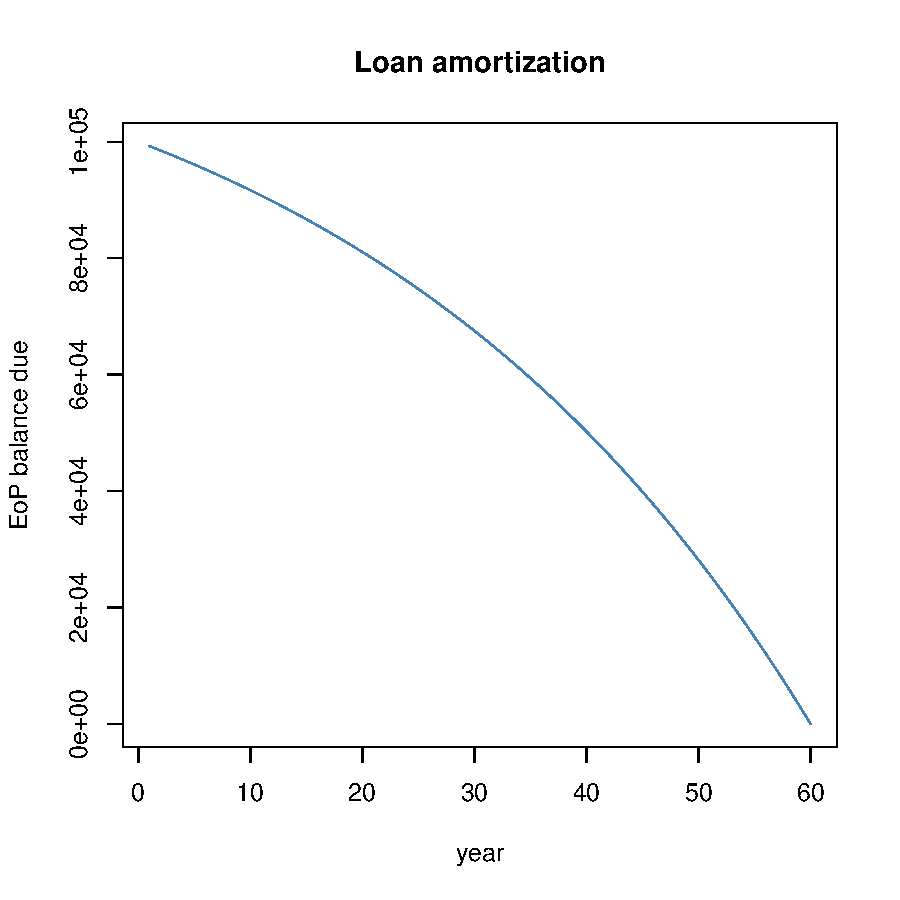
\includegraphics{an_introduction_to_lifecontingencies_package-figBalanceDue}
\caption{Loan amortization: EoP balance due.}
\label{fig:LoanAmort}
\end{center}
\end{figure}


\subsubsection{Bond pricing}\label{sss:finbond}

Bond pricing represents another application of present value. A standard bond
with face value $C$ and term length $T$ consists of
equal coupons $c$ paid at regular intervals. The final payment at time $T$ is 
$C_T + c$.
Equation~\ref{eq:bond} expresses the present value of a bond with $n$ remaining
coupons.

\begin{equation}
B = {c}*{a}_{\left. {\overline {\, n \,}}\! \right| } + {C}*{v^{T}}
	\label{eq:bond}
\end{equation}


Perpetuities are financial contracts that offer an indefinite sequence of
payments either at the end (perpetuity-immediate) or at the beginning of each
period (perpetuity-due).\\

The following examples show how elementary functions in the  \pkg{lifecontingencies} package can be combined to price bonds and perpetuities.
\begin{Schunk}
\begin{Sinput}
R> bond<-function(faceValue, couponRate, couponsPerYear, yield,maturity)
+  {
+  	out <- numeric(1)
+  	numberOfCF <- maturity * couponsPerYear
+  	CFs <- numeric(numberOfCF)
+  	payments <- couponRate * faceValue / couponsPerYear 
+  	cf <- payments * rep(1,numberOfCF)
+  	cf[numberOfCF] <- faceValue + payments 
+  	times <- seq.int(from=1/couponsPerYear, to=maturity, 
+                  by=maturity/numberOfCF)
+  	out <- presentValue(cashFlows=cf, interestRates=yield, 
+                     timeIds=times)
+  	return(out)
+  }
R> perpetuity<-function(yield, immediate=TRUE)
+  {
+  	out <- numeric(1)
+  	out <- 1 / yield
+  	out <- ifelse(immediate==TRUE, out, out*(1+yield))
+  	return(out)
+  }
R> 
\end{Sinput}
\end{Schunk}

As displayed below, the \code{bond} and \code{perpetuity} functions defined above can be used to price
any bond, given face value, coupon rate, and term.

\begin{Schunk}
\begin{Sinput}
R> bndEx1 <-bond(1000, 0.06, 2, 0.05, 3)
R> bndEx2 <-bond(1000, 0.06, 2, 0.06, 3)
R> ppTy1 <-perpetuity(0.1)
R> c(bndEx1, bndEx2, ppTy1)
\end{Sinput}
\begin{Soutput}
[1] 1029.250 1002.371   10.000
\end{Soutput}
\end{Schunk}


\subsubsection{Duration and ALM}\label{sss:DurationAndAlm}


As defined within the package, duration and convexity formulas are reported in
Equation~\ref{eq:duration} and Equation~\ref{eq:convexity} respectively. Their typical application lies within
porfolios' asset - liability management (ALM).
The interested reader can find details
in \cite{mathFinAct} and \cite{broverman2008mathematics} textbooks.
However, the following example shows how the Macaulay duration
(\code{ex1}), modified duration (\code{ex2}), and convexity (\code{ex3}) of any series of cash flows can 
be calculated by \pkg{lifecontingencies} package functions.\\

\begin{equation}
D = \sum\limits_t^{T} \frac{t*\text{CF}_{t} \left( 1 + \frac{i}{m} \right)^{
- t * m}}{P}
\label{eq:duration}
\end{equation}


\begin{equation}
C = \sum\limits_{t}^{T} t * \left( t +
\frac{1}{m} \right) * \text{CF}_{t} \left( 1 + \frac{y}{m} \right)^{ - m * t - 2}
\label{eq:convexity}
\end{equation}

\begin{Schunk}
\begin{Sinput}
R> cashFlows <- c(100,100,100,600,500,700)
R> timeVector <- seq(1:6)
R> interestRate <- 0.03
R> dur1 <-duration(cashFlows = cashFlows, timeIds = timeVector, 
+  		i = interestRate, k = 1, macaulay = TRUE)
R> dur2 <-duration(cashFlows = cashFlows, timeIds = timeVector, 
+  		i = interestRate, k = 1, macaulay = FALSE)
R> cvx1 <-convexity(cashFlows = cashFlows, timeIds = timeVector, 
+  		i = interestRate, k = 1)
R> c(dur1, dur2, cvx1)
\end{Sinput}
\begin{Soutput}
[1]  4.430218  4.563124 25.746469
\end{Soutput}
\end{Schunk}

This example works out a small ALM problem. Suppose an insurance company has
sold a guaranteed term certificate (GTC) with face value \$ 10,000 that will
mature in 7 years at an interest rate of 5\% . Its final value would be:

\begin{Schunk}
\begin{Sinput}
R> GTCFin<- 10000 * (1 + 0.05)^7
R> GTCFin
\end{Sinput}
\begin{Soutput}
[1] 14071
\end{Soutput}
\end{Schunk}

Imagine the company can hedge its liability with two available investment
instruments:
\begin{enumerate}
  \item A five year bond with face value of 100 and 3\% coupons paid annually.
  \item A perpetuity-immediate. As a remark, the formulas for the PV,
  duration and convexity of a perpetuity immediate are $PV_{\text{pp}}=\frac{1}{y}$, 
  $D_{\text{pp}}=\frac{1+y}{y}$, $C_{\text{pp}}=\frac{2}{y^2}$ respectively, if the yield rate is $y$.
 \end{enumerate}
Assume the issuing company wants to hedge its liability with an investment
portfolio that will not be affected adverserly by changes in the investment yield. In order to solve
the ALM problem, the composition of assets within the portfolio shall be
chosen accordingly. Moreover, assume that the current market yield rate is 4\%. The following lines of code figure out some parameters that are used within the
example.

\begin{Schunk}
\begin{Sinput}
R> yieldT0 <- 0.04
R> durLiab <- 7
R> pvLiab <- presentValue(cashFlows = GTCFin,timeIds = 7,
+  		interestRates = yieldT0)
R> convLiab <- convexity(cashFlows=GTCFin, timeIds = 7, 
+  		i=yieldT0)
R> pvBond <- bond(100,0.03,1,yieldT0,5)
R> durBond <- duration(cashFlows=c(3,3,3,3,103), 
+  		timeIds=seq(1,5), i = yieldT0)
R> convBond <- convexity(cashFlows=c(3,3,3,3,103), 
+  		timeIds=seq(1,5), i = yieldT0)
R> pvPpty <- perpetuity(yieldT0)
R> durPpty <- (1+yieldT0)/yieldT0
R> covnPpty <- 2/(yieldT0^2)
\end{Sinput}
\end{Schunk}

Then the ALM problem can be set up as a three step problem, as the \cite{mathFinAct}
texbook remarks:
\begin{enumerate}
  \item Setting the initial present value of cash inflows (assets) to be equal
  to the present value of cash outflows (liabilities). 
  \item Setting the interest rate sensitivity (i.e., the duration) of assets to
  be equal to the interest rate sensitivity of liabilities. This is done by solving
  the system of equations shown in Equation~\ref{eq:alm2}. The parameters $w_i$ and $D_i$
 stand for asset hedging weights and duration values
  respectively.
  \begin{equation}
  \left\{ \begin{array}{l}
    {w_{\text{bnd}}}{D_{\text{bnd}}} + {w_{\text{ppt}}}{D_{\text{ppt}}} = D_{\text{GTC}}\\
    w_{\text{bnd}} + w_{\text{ppt}} = 1
    \end{array} \right.
  \label{eq:alm2}
\end{equation}
 \item Setting the convexity of assets to be greater than the convexity  of liabilities. In other words, this means verifying that asset decline
 (growth) will be slower (faster) than liability decline in case of a change in the 
 interest rate.
\end{enumerate}

The following lines of code calculate the asset weights vector by linear algebra
functions bundled in \proglang{R} base.

\begin{Schunk}
\begin{Sinput}
R> a <- matrix(c(durBond, durPpty,1,1), nrow=2, 
+  		byrow=TRUE)
R> b <- as.vector(c(7,1))
R> weights <-solve(a,b)
R> weights
\end{Sinput}
\begin{Soutput}
[1] 0.8848879 0.1151121
\end{Soutput}
\end{Schunk}

Vector \code{weights} displays the portfolio composition in terms of bonds and
perpetuities, respectively. Therefore, the number of bonds and perpetuities that
can be purchased is determined by: 

\begin{Schunk}
\begin{Sinput}
R> bondNum <- weights[1] * pvLiab / pvBond
R> pptyNum <- weights[2] * pvLiab / pvPpty	
R> bondNum
\end{Sinput}
\begin{Soutput}
[1] 99.0279
\end{Soutput}
\begin{Sinput}
R> pptyNum
\end{Sinput}
\begin{Soutput}
[1] 49.23485
\end{Soutput}
\end{Schunk}

It can be verified that the convexity of assets is greater than the convexity of liabilities.

\begin{Schunk}
\begin{Sinput}
R> convAsset <- weights[1] * convBond + weights[2] * covnPpty
R> convAsset>convLiab
\end{Sinput}
\begin{Soutput}
[1] TRUE
\end{Soutput}
\end{Schunk}

The portfolio is immunized from yield rate variations because the present value of assets will be greater than the present value of the liabilities if the interest rate
suddently drops to 3\% just after hedging the asset purchase. The same occurs in case of an upward shift in the interest rate
toward 5\%.

\begin{Schunk}
\begin{Sinput}
R> yieldT1low <- 0.03
R> immunizationTestLow <- (bondNum * bond(100,0.03,1,yieldT1low,5) + 
+  			pptyNum * perpetuity(yieldT1low)> 
+  			GTCFin / (1+yieldT1low)^7)
R> yieldT1high <- 0.05
R> immunizationTestHigh <- (bondNum * bond(100,0.03,1,yieldT1high,5) + 
+  			pptyNum * perpetuity(yieldT1high)>
+  			GTCFin/(1+yieldT1high)^7)
R> immunizationTestLow
\end{Sinput}
\begin{Soutput}
[1] TRUE
\end{Soutput}
\begin{Sinput}
R> immunizationTestHigh
\end{Sinput}
\begin{Soutput}
[1] TRUE
\end{Soutput}
\end{Schunk}

It is worthwhile to remember that asset allocation within the portfolio should
be rebalanced with some frequency, since the portfolio's duration
and convexity will change as time goes on.


\subsection{Analysis of life tables and actuarial tables}\label{ss:lfActT}

\begin{table}[h]
\centering
\begin{tabular}{ll}
  \hline
	Function & Purpose\\
      \hline  \hline
	\code{dxt} & deaths between age $x$ and $x+t$, ${}_{t}d_{x}$.\\
	\code{pxt} & survival probability between age $x$ and $x+t$, ${}_{t}p_{x}$.\\
	\code{pxyzt} & survival probability for two (or more) lives, ${}_{t}p_{xy}$.\\
	\code{qxt} & death probability between age $x$ and $x+t$, ${}_{t}q_{x}$.\\
	\code{qxyzt} & death probability for two (or more) lives, ${}_{t}q_{xy}$.\\
	\code{Txt} & number of person-years lived after exact age $x$, ${}_{t}T_{x}$.\\
	\code{mxt} & central death rate, ${}_{t}m_{x}$.\\
		\code{qx2mx} & convert death probabilities into mortality rate.\\
		\code{mx2qx} & convert mortality rate into death probabilities. \\
	\code{exn} & expected lifetime between age $x$ and age $x + n$,
	${}_{n}e_{x}$.\\
	\code{rLife} & sample from the time until death distribution underlying 
	a life table.\\
    \code{rLifexyz} & sample from the time until death distribution underlying 
	 two or more lives.\\
	\code{exyz} &  n-year curtate lifetime of the joint-life status.\\
	\code{probs2lifetable}  &  life table $l_x$ from raw one - year survival / death probabilities.\\
      \hline
\end{tabular}
\caption{\pkg{lifecontingencies} functions for demographic analysis.}
\label{tab:demofun}
\end{table}



\code{lifetable} and \code{actuarialtable} classes are designed to handle demographic and actuarial mathematics calculations. An \code{actuarialtable} class inherits
from \code{lifetable} class; it adds one more slot for the rate
of interest. Both classes have been designed using the \code{S4} \proglang{R}
classes framework.\\
Table~\ref{tab:demofun} lists the functions that have been developed for performing
demographic analysis within \pkg{lifecontingencies} package. This section
briefly exemplifies these functions.

\subsubsection{Creating lifetable and actuarialtable objects}\label{sss:creating}
Life table objects can be created by using either raw \proglang{R} commands or existing \code{data.frame} objects.
However, three components are needed to build a \code{lifetable} class object:
\begin{enumerate}
	\item The years sequence, which is an integer sequence $0,1,\ldots, \omega$. It shall 
	start from zero and end at $\omega$, the terminal age (the age $x$
	for which $p_x=0$).
	\item The $l_x$ vector, which is the number of subjects living at the beginning
	of age $x$; in other words, the number of subjects at risk of dying between year
	$x$ and $x+1$.
	\item The name of the life table.
\end{enumerate}

There are three main approaches for creating a \code{lifetable} object:
\begin{enumerate}
	\item Directly from the $x$ and $l_x$ vector.
	\item By importing $x$ and $l_x$ from an existing \code{data.frame} object.
	\item From using raw survival probabilities.
\end{enumerate}

Creating a \code{lifetable} object directly can be done as shown by the code
below:

\begin{Schunk}
\begin{Sinput}
R> x_example <- seq(from=0,to=9, by=1)
R> lx_example <- c(1000,950,850,700,680,600,550,400,200,50)
R> exampleLt <- new("lifetable", x=x_example, lx=lx_example, 
+  		name="example lifetable")
\end{Sinput}
\end{Schunk}

\code{print} and \code{show}  methods tabulate 
the $x$, $l_x$, ${}_{t}p_{x}$ and $e_x$ values for a given life table.


\begin{Schunk}
\begin{Sinput}
R> print(exampleLt)
\end{Sinput}
\begin{Soutput}
Life table example lifetable 

  x   lx        px       ex
1 0 1000 0.9500000 4.980000
2 1  950 0.8947368 4.242105
3 2  850 0.8235294 3.741176
4 3  700 0.9714286 3.542857
5 4  680 0.8823529 2.647059
6 5  600 0.9166667 2.000000
7 6  550 0.7272727 1.181818
8 7  400 0.5000000 0.625000
9 8  200 0.2500000 0.250000
\end{Soutput}
\end{Schunk}

\code{head} and \code{tail} methods for \code{data.frame} S3 classes have also 
been implemented on \code{lifetable} classes.

\begin{Schunk}
\begin{Sinput}
R> head(exampleLt)
\end{Sinput}
\begin{Soutput}
  x   lx
1 0 1000
2 1  950
3 2  850
4 3  700
5 4  680
6 5  600
\end{Soutput}
\end{Schunk}

Still, the easiest way to create a \code{lifetable} object is to start 
from a suitable existing \code{data.frame}. This will probably be the most
practical approach for practicing actuaries. Some life or mortality rate
tables have been bundled within the \pkg{lifecontingencies} package, as
Table~\ref{tab:lifeTables} displays.


\begin{table}[h]
\centering
\begin{tabular}{ll}
\hline
	Data set & Description\\
 \hline \hline
    \code{AF92Lt} & UK AF92 life table.\\
    \code{AM92Lt} & UK AF92 life table.\\
    \code{demoChina} & China mortality rates from SOA website.\\
	\code{demoIta} & Various Italian life tables including RG48 and IPS55 projected
	tables.\\
    \code{demoJapan} & Japan mortality rates from SOA website.\\
    \code{demoUsa} & US Social Security life tables.\\
    \code{demoFrance} & 1990 and 2002 French life tables.\\
    \code{demoCanada} & UP94 (standard, 2015, 2020) mortality rates for males and females.\\
    \code{soa08} & SOA illustrative life table.\\
    \code{soa08Act} & SOA illustrative actuarial table at
    6\%.\\    
 \hline
\end{tabular}
\caption{Life tables and other data objects bundled
within \pkg{lifecontingencies}.}
\label{tab:lifeTables}
\end{table}

The following example shows how US Social Security life tables are loaded
from the existing \code{demoUsa} data set bundled in the \pkg{lifecontingencies} package.

\begin{Schunk}
\begin{Sinput}
R> data("demoUsa")
R> data("demoIta") 
R> usaMale07 <- demoUsa[,c("age", "USSS2007M")]
R> usaMale00 <- demoUsa[,c("age", "USSS2000M")]
R> names(usaMale07) <- c("x","lx")
R> names(usaMale00) <- c("x","lx")
R> usaMale07Lt <-as(usaMale07,"lifetable")
R> usaMale07Lt@name <- "USA MALES 2007"
R> usaMale00Lt <-as(usaMale00,"lifetable")
R> usaMale00Lt@name <- "USA MALES 2000"
\end{Sinput}
\end{Schunk}

The same operation can be performed on IPS55 tables bundled in the \code{demoIta} data set. The purpose of the 
following example is to stress the importance of using a clean $l_x$ series as an input for the coerce method. A "clean" 
$l_x$ series is a decreasing series without zeroes or missing values.

\begin{Schunk}
\begin{Sinput}
R> lxIPS55M <- with(demoIta, IPS55M)
R> pos2Remove <- which(lxIPS55M %in% c(0,NA))
R> lxIPS55M <-lxIPS55M[-pos2Remove]
R> xIPS55M <-seq(0,length(lxIPS55M)-1,1)
R> ips55M <- new("lifetable",x=xIPS55M, lx=lxIPS55M, 
+  		name="IPS 55 Males")
R> lxIPS55F <- with(demoIta, IPS55F)
R> pos2Remove <- which(lxIPS55F %in% c(0,NA))
R> lxIPS55F <- lxIPS55F[-pos2Remove]
R> xIPS55F <- seq(0,length(lxIPS55F)-1,1)
R> ips55F <- new("lifetable",x=xIPS55F, lx=lxIPS55F, 
+  		name="IPS 55 Females")
\end{Sinput}
\end{Schunk}


The final method of creating a \code{lifetable} object uses 
one year survival or death probabilities, combining the \code{probs2lifetable} function with 
\code{as.data.frame} coerce methods. Two potential benefits arise from using this function. The first benefit lies in the use of mortality projection method
results. The Lee - Carter method \citep{Lee1992} allows one to vary mortality table
by cohort of birth.
Thus, demographic quantities, like the expected lifetime, $e_0$,can be projected as functions of the year of birth.\\
A second advantage lies in the creation of "cut-down" mortality tables. This latter
application is exemplified in the code that follows, where a \code{itaM2002reduced} life
table is obtained; the one - year mortality rates of Italian males aged between 20 and 60 are cut down to 20\% of their original value.

\begin{Schunk}
\begin{Sinput}
R> data("demoIta")
R> itaM2002 <- demoIta[,c("X","SIM92")]
R> names(itaM2002) <- c("x","lx")
R> itaM2002Lt <- as(itaM2002,"lifetable")
\end{Sinput}
\begin{Soutput}
removing NA and 0s
\end{Soutput}
\begin{Sinput}
R> itaM2002Lt@name <- "IT 2002 Males"
R> itaM2002 <- as(itaM2002Lt,"data.frame")
R> itaM2002$qx <- 1-itaM2002$px
R> for(i in 20:60) itaM2002$qx[itaM2002$x==i] = 0.2 * itaM2002$qx[itaM2002$x==i]
R> itaM2002reduced <- probs2lifetable(probs=itaM2002[,"qx"], radix=100000,
+  		type="qx",name="IT 2002 Males reduced")
\end{Sinput}
\end{Schunk}


An \code{actuarialtable} can be easily created from an existing \code{lifetable} object.

\begin{Schunk}
\begin{Sinput}
R> exampleAct <- new("actuarialtable",x=exampleLt@x, lx=exampleLt@lx, 
+  interest=0.03, name="example actuarialtable")
\end{Sinput}
\end{Schunk}

When applied to
either \code{actuarialtable} or \code{lifetable} classes, Method \code{getOmega}  returns the terminal age, $\omega$.

\begin{Schunk}
\begin{Sinput}
R> getOmega(exampleAct)
\end{Sinput}
\begin{Soutput}
[1] 9
\end{Soutput}
\end{Schunk}

Method \code{print} behaves differently for \code{lifetable} and 
\code{actuarialtable} objects. In fact, when the \code{print} method is applied on a
\code{lifetable} object, it tabulates both the one year survival probability and the complete
expected remaining life until death. Conversely, when the \code{print} method is
applied on a \code{lifetable} object, classical commutation
functions ($D_x$, $N_x$, $C_x$, $M_x$, $R_x$), discussed later, are printed out.

\begin{Schunk}
\begin{Sinput}
R> print(exampleLt)
\end{Sinput}
\begin{Soutput}
Life table example lifetable 

  x   lx        px       ex
1 0 1000 0.9500000 4.980000
2 1  950 0.8947368 4.242105
3 2  850 0.8235294 3.741176
4 3  700 0.9714286 3.542857
5 4  680 0.8823529 2.647059
6 5  600 0.9166667 2.000000
7 6  550 0.7272727 1.181818
8 7  400 0.5000000 0.625000
9 8  200 0.2500000 0.250000
\end{Soutput}
\begin{Sinput}
R> print(exampleAct)
\end{Sinput}
\begin{Soutput}
Actuarial table  example actuarialtable interest rate  3 % 

   x   lx         Dx         Nx        Cx       Mx        Rx
1  0 1000 1000.00000 5467.92787  48.54369 840.7400 4839.7548
2  1  950  922.33010 4467.92787  94.25959 792.1963 3999.0148
3  2  850  801.20652 3545.59778 137.27125 697.9367 3206.8185
4  3  700  640.59916 2744.39125  17.76974 560.6654 2508.8819
5  4  680  604.17119 2103.79209  69.00870 542.8957 1948.2164
6  5  600  517.56527 1499.62090  41.87421 473.8870 1405.3207
7  6  550  460.61634  982.05563 121.96373 432.0128  931.4337
8  7  400  325.23660  521.43929 157.88185 310.0491  499.4210
9  8  200  157.88185  196.20268 114.96251 152.1672  189.3719
10 9   50   38.32084   38.32084  37.20470  37.2047   37.2047
\end{Soutput}
\end{Schunk}

It is possible to convert the \code{actuarialtable} object into a
\code{data.frame} object, as shown below.

\begin{Schunk}
\begin{Sinput}
R> exampleActDf <- as(exampleAct, "data.frame")
\end{Sinput}
\end{Schunk}

A recent \pkg{lifecontingencies} package enhancement allows to export a life
table as non - homogeneous discrete Markov chain by means of
\code{markovchainList} S4 class object as defined in \pkg{markovchain}
\citep{markovchainR} \proglang{R} package.

\begin{Schunk}
\begin{Sinput}
R> data(soa08)
R> require(markovchain)
R> soa08Mc<-as(soa08,"markovchainList")
\end{Sinput}
\end{Schunk}

Finally, a \code{plot} method can be applied to either\code{lifetable} or
\code{actuarialtable} objects. The underlying survival function (which is the plot of $x$ vs $l_x$) is displayed in both cases. 
Figure~\ref{fig:SoaLt} shows the \code{plot} methods applied on a Society of
Actuaries (SOA) actuarial table at 6\% interest, which comes bundled within the
\pkg{lifecontingencies} package as \code{soa08Act} object.



\begin{figure}
\begin{center}
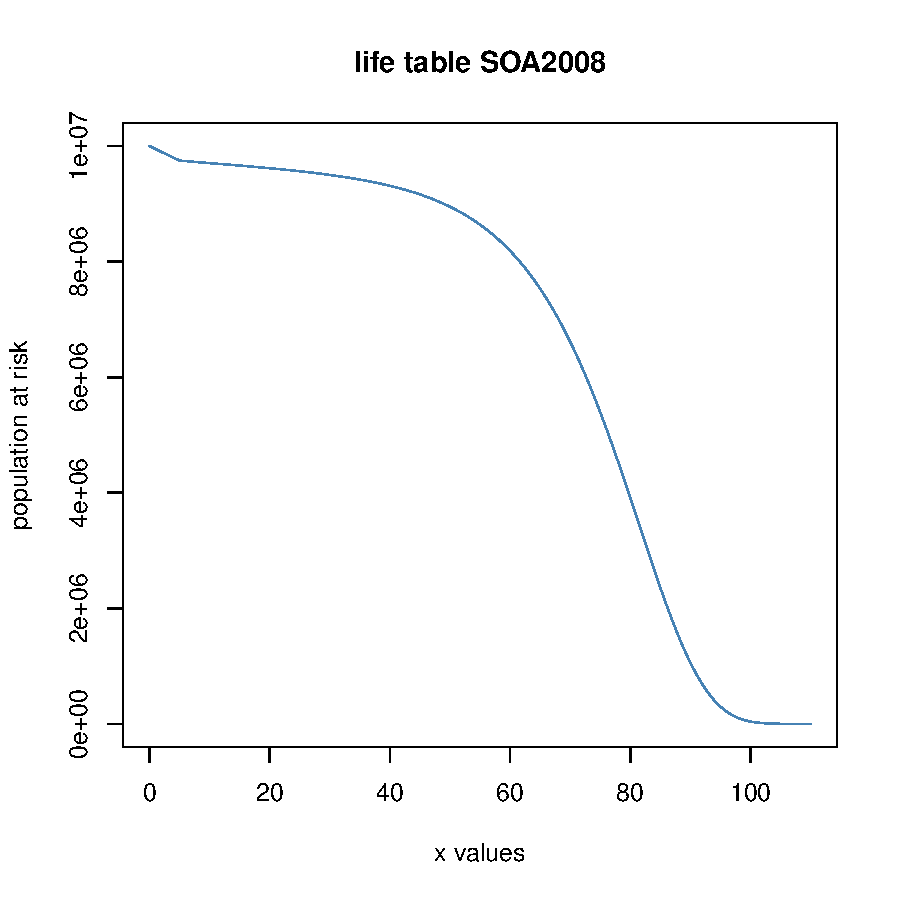
\includegraphics{an_introduction_to_lifecontingencies_package-figSurvivalFunction}
\caption{Underlying survival function of SOA illustrative life table.}
\label{fig:SoaLt}
\end{center}
\end{figure}

\clearpage

\subsubsection{Basic demographic analysis}\label{sss:demograph}

Basic demography calculations can be performed on 
valid \code{lifetable} or \code{actuariatable} objects. The functions discussed in this section calculate proper ratios or sums on $l_x$ or $d_x$ values using functions that access to the lifetable object slots. This is all done in accordance with the demographic formula definitions.\\


The code below shows how ${}_{1}p_{20}$, ${}_{2}q_{30}$ and $\mathring{e}_{50:\lcroof{20}}$
are calculated respectively on the IPS55 male population table 

\begin{Schunk}
\begin{Sinput}
R> demoEx1<-pxt(ips55M,20,1)
R> demoEx2<-qxt(ips55M,30,2) 
R> demoEx3<-exn(ips55M, 50,20,"complete") 
R> c(demoEx1,demoEx2,demoEx3)
\end{Sinput}
\begin{Soutput}
[1]  0.999595096  0.001332031 19.472765230
\end{Soutput}
\end{Schunk}

Getting mortality rates and moving to death probabilities is also possible

\begin{Schunk}
\begin{Sinput}
R> mx20t1 <- mxt(ips55M,20,1)
R> qx20t1 <- mx2qx(mx20t1)
R> c(mx20t1,qx20t1)
\end{Sinput}
\begin{Soutput}
[1] 0.0004049862 0.0004049042
\end{Soutput}
\end{Schunk}

The package allows one to calculate fractional survival
probabilities through the use of linear interpolation, constant force of mortality and hyperbolic 
Balducci's assumptions as shown by the code below.\\

\begin{Schunk}
\begin{Sinput}
R> data("soa08Act")
R> pxtLin <- pxt(soa08Act,80,0.5,"linear") 
R> pxtCnst <- pxt(soa08Act,80,0.5,"constant force") 
R> pxtHyph <- pxt(soa08Act,80,0.5,"hyperbolic") 
R> c(pxtLin,pxtCnst,pxtHyph)
\end{Sinput}
\begin{Soutput}
[1] 0.9598496 0.9590094 0.9581701
\end{Soutput}
\end{Schunk}

Calculations for survival probabilities on two (or more) lives can also be performed.
 As a remark, two different life statuses are defined within the analysis of multiple lives
survival: "joint" survival status and "last" survival status. The
"joint" survival status exists while all the members of the pool are alive,
while the "last" survival status exists until the last member of the pool dies.
All calculations assume that the multiple lives are independent.
Equation~\ref{eq:2headssurv} expresses the remaining future lifetime on a couple $xy$ under the joint and last survival status
respectively. 

\begin{equation}
\begin{gathered}
  \tilde T_{xy} = \min \left( T_x,T_y \right) \hfill \\
  \tilde T_{\bar{xy}} = \max \left( T_x,T_y \right) \hfill \\ 
\end{gathered}
\label{eq:2headssurv}
\end{equation}


The following code shows how the joint survival probability, last survival probability, and 
expected joint lifetime can be evaluated using functions in  \pkg{lifecontingencies}.

\begin{Schunk}
\begin{Sinput}
R> tablesList <- list(ips55M, ips55F)
R> jsp <- pxyzt(tablesList, x=c(65,63), t=2)
R> lsp <- pxyzt(tablesList, x=c(65,63), t=2, status="last") 
R> jelt <- exyzt(tablesList, x=c(65,63), status="joint") 
R> c(jsp,lsp,jelt)
\end{Sinput}
\begin{Soutput}
[1]  0.9813187  0.9999275 19.1982972
\end{Soutput}
\end{Schunk}

\subsection{Classical actuarial mathematics examples}\label{ss:actMath}
\begin{table}[h]
\centering
\begin{tabular}{lll}
  \hline
	Function & Purpose & APV symbol\\
      \hline   \hline
	\code{Axn} & one  life insurance & $\termins{x}{n}$.\\
	\code{AExn} & the n-year  endowment & $\pureend{x}{n}$.\\
	\code{Axyzn} & two lives life insurances &
	$\lcterm{\bar{A}}{\overline{xy}}{n}$.\\
	\code{axn} & one life annuity & $\ddot{a}_x$.\\
	\code{axyzn} & two lives annuities & $\ddot{a}_{xy}$.\\
	\code{Exn} & pure endowment & $\pureendc{x}{n}$.\\
	\code{Iaxn} & increasing annuity & $Ia_{x}$.\\
	\code{IAxn} & increasing life insurance & $\lcterm{(IA)}{x}{n}$.\\
	\code{DAxn} & decreasing life insurance &  $\lcterm{(DA)}{x}{n}$.\\
    \code{rLifeContingencies} & generates variates from the $\tilde Z$ distribution.\\
    \code{rLifeContingenciesXyz} & multiple lives version of \code{rLifeContingencies}.\\
      \hline
\end{tabular}
\caption{\pkg{lifecontingencies} functions for actuarial mathematics.}
\label{tab:actfun}
\end{table}

Table~\ref{tab:actfun} lists examples of functions contained in \pkg{lifecontingencies} that allow the user to perform classical actuarial mathematics
calculations. In the selection of examples that follow, the SOA illustrative life table with an interest rate of 6\% will be used unless otherwise stated

\subsubsection{Life insurance examples}\label{sss:lifeInsurances}


The evaluation of the APV has traditionally followed one of three approaches: the use of commutation tables, the current payment technique, or the expected value method.\\ 
Commutation tables extend the life table by tabulating special functions of age and
rate of interest, as \cite{anderson1999commutation} further considers.
Ratios of commutation table functions allow an actuary to evaluate APV for standard insurances. However, commutation table usage has become less prominent in the computer era. In fact, these tables are not flexible enough and their
usage is computationally inefficient. Therefore, the \pkg{lifecontingencies} package does not use the commutation table approach to evaluate APVs.\\
The current payment technique calculates the APV of a life contingency
insurance, $\bar Z$, as the scalar product of three vectors:
$\bar Z = \left\langle {\left\langle {\bar c \bullet \bar v} \right\rangle  \bullet \bar p} \right\rangle$; this uses the vector of all possible uncertain cash flows, $\bar c$, 
the vector of discount factors, $\bar v$, and the vector of cash flow
probabilities, $\bar p$. The \pkg{lifecontingencies} package implements the current
payment technique by using actuarial functions listed in Table~\ref{tab:actfun} to
evaluate APVs. Finally, the expected value approach models $\bar Z$ as the
scalar product of two vectors: $\bar Z = \left\langle \bar{pk} \bullet \bar x \right\rangle$. $\bar{pk}$ is $Pr \left[ \tilde K = k \right]$, the probability that the future curtate lifetime will be exactly $k$ years, where $\bar x$ is the present value of benefits due under the policy term if $\tilde K = k$.
\code{rLifeContingencies} and \code{rLifeContingenciesXyz} implement the
expected value approach to generate $\tilde Z$ variates.\\

Consider an $n$ year annuity due. Its APV, $\anndue{x}{n}$, using
the commutation table approach is reported in Equation~\ref{eq:anndueComm}, while Equation~\ref{eq:anndueCVA} reports the same APV using the current payment technique. Finally, Equation~\ref{eq:anndueEVT} calculates the APV using the expected value approach.

\begin{equation}
	\text{APV} = \frac{N_x - N_{x + n}}{D_x}
	\label{eq:anndueComm}
\end{equation}   

\begin{equation}
\text{APV} = \sum\limits_{k = 0}^{\min \left( \omega  - x ,n \right)} {{}_{k}p_{x}*v^{k}} 
	\label{eq:anndueCVA}
\end{equation}

\begin{equation}
\text{APV} = \sum\limits_{k = 0}^{\omega  - x} {\Pr \left[ \tilde K_x = k \right]*{\ddot a_{\left. {\overline {\, 
 {\min \left( k, n \right)} \,}}\! \right| }}} 
 \label{eq:anndueEVT}
\end{equation}

In order to understand how \pkg{lifepackage} implements the current
payment technique in its actuarial function, it is worthwhile to look closer at the core of the
\code{axn} function. This function takes the following parameters as
inputs: \code{n}, the term of the annuity; \code{k} the fractional payment frequency; 
\code{x} the annuitant age; \code{m}, the deferring period. Then, it defines:
\begin{enumerate}
  \item The vector of possible payments, $\bar{c}$, by
    \begin{Code}
     payments = rep(1/k, n * k)
    \end{Code}
  \item The vector timing of payments, by
     \begin{Code}
     times=m + seq(from=0, to=(n-1/k), by=1/k)
     \end{Code}
   \item The vector of payment probability, $\bar{p}$, by
     \begin{Code}
     for(i in 1:length(times)) probs[i] = pxt(
     actuarialtable, x,times[i])
     \end{Code}
   \item Finally, the three vectors are passed as input parameters to the
   \code{presentValue} function as the following code shows:
   \begin{Code}
     presentValue(cashFlows=payments, timeIds=times, 
     interestRates = interest,
     probabilities=probs)
   \end{Code}
\end{enumerate}


In the examples that follow, the SOA illustrative actuarial 
table is used in the calculation of premiums and reserves of life contingencies.\\

The first example values a 40-year insurance on a policyholder aged 25,
with benefits payable at the end of the month of death. Equation~\ref{eq:lifeInsComm} would determine the
benefit premium using the commutation table approach.

\begin{equation}
U = \frac{M_{25} - M_{65}}{{{D_{65}}}}\frac{i}{{{i^{\left( {12}
\right)}}}}
\label{eq:lifeInsComm}
\end{equation}

The following lines of code compute the benefit premium using
\code{UComm}, the commutation technique, and \code{UCpt}, the current payment technique.

\begin{Schunk}
\begin{Sinput}
R> data(soa08Act)
R> UComm <- Axn(actuarialtable=soa08Act, x=25, n=65-25, k=12)
R> UCpt <- ((soa08ActDf$Mx[26]-soa08ActDf$Mx[66])/soa08ActDf$Dx[26]) * 
+  		0.06/real2Nominal(i=0.06,k=12)
R> c(UComm, UCpt)
\end{Sinput}
\begin{Soutput}
[1] 0.04927622 0.04927622
\end{Soutput}
\end{Schunk}

If, while the policyholder is alive, the premium is paid in ten equal installments at the beginning of each year instead of a lump sum, then the yearly premium, $P$ , would be determined  as follows:

\begin{Schunk}
\begin{Sinput}
R> P <- UCpt/axn(actuarialtable=soa08Act,x=25,n=10)
R> P
\end{Sinput}
\begin{Soutput}
[1] 0.006351049
\end{Soutput}
\end{Schunk}

The \pkg{lifecontingencies} package allows one to evaluate APVs of endowment insurances; this can be calculated for increasing and decreasing life insurances as well. The lines of code that follow will
 prove the actuarial equivalence expressed by
Equation~\ref{eq:decreaseIncrease} in a computational context.

\begin{equation}
\left( n + 1 \right) * \termins{x}{n} = \lcterm{(DA)}{x}{n} + \lcterm{(IA)}{x}{n} 
\label{eq:decreaseIncrease}
\end{equation}

\begin{Schunk}
\begin{Sinput}
R> (10 + 1 ) * Axn(actuarialtable=soa08Act, x=25, n=10) 
\end{Sinput}
\begin{Soutput}
[1] 0.1194393
\end{Soutput}
\begin{Sinput}
R> DAxn(actuarialtable = soa08Act, x=25, n=10) + 
+  IAxn(actuarialtable = soa08Act, x=25, n=10)
\end{Sinput}
\begin{Soutput}
[1] 0.1194393
\end{Soutput}
\end{Schunk}


\subsubsection{Life annuity examples}\label{sss:annuities}
Life contingent annuities form sequences of payments whose occurrence 
and duration depend the policyholder's future lifetime. The few examples that follow demonstrate how the \pkg{lifecontingencies} package can directly compute the APV for typical life contingencies using either bundled functions or classical commutation tables.\\


Equation~\ref{eq:ann1} expresses the full premium of a ten-year deferred
annuity-due for a policyholder aged 75 by means of commutation functions.

\begin{equation}
U={}_{10|}\ddot{a}_{75}=\frac{N_{85}}{D_{75}}
\label{eq:ann1}
\end{equation}

\begin{Schunk}
\begin{Sinput}
R> UCpt <- axn(actuarialtable=soa08Act, x=75, m=10)
R> UComm <- with(soa08ActDf,Nx[86]/Dx[76])
R> c(UCpt,UComm)
\end{Sinput}
\begin{Soutput}
[1] 1.146484 1.146484
\end{Soutput}
\end{Schunk}

If the premium were paid by means of five annual payments as long as the insured were alive, Equation~\ref{eq:ann1} would be rewritten as Equation~\ref{eq:ann2}.

\begin{equation}
{}_{5}{P}({}_{10|}\ddot{a}_{75})=\frac{{}_{10|}\ddot{a}_{75}}{\ddot{a}_{75:\lcroof{5}}}=\frac{{\frac{{{N_{85}}}}{{{D_{75}}}}}}{{\frac{{{N_{75}} - {N_{80}}}}{{{D_{75}}}}}}
\label{eq:ann2}
\end{equation}

\begin{Schunk}
\begin{Sinput}
R> P=axn(actuarialtable=soa08Act, x=75, m=10) / 
+  		axn(actuarialtable=soa08Act, x=75, n=5)
R> P
\end{Sinput}
\begin{Soutput}
[1] 0.2854726
\end{Soutput}
\begin{Sinput}
R> PComm <- with(soa08ActDf,(Nx[86]/Dx[76]) / 
+  				((Nx[76]-Nx[81])/Dx[76]))
R> PComm
\end{Sinput}
\begin{Soutput}
[1] 0.2854726
\end{Soutput}
\end{Schunk}

If amounts of $\frac{1}{m}$ were paid at the beginning of each month,  the
APV of the annuty would be $U={}_{10|}\ddot{a}_{75}^{(12)}$.




\begin{Schunk}
\begin{Sinput}
R> U <- axn(actuarialtable=soa08Act, x=75, m=10, k=12)
R> P <- axn(actuarialtable=soa08Act, x=75, m=10, k=12) / 
+  		axn(actuarialtable=soa08Act, x=75, n=5)
R> c(U,P)
\end{Sinput}
\begin{Soutput}
[1] 1.0325685 0.2571079
\end{Soutput}
\end{Schunk}




\subsubsection{Benefit reserves examples}\label{sss:benefitReserves}

The (prospective) benefit reserve consists in the difference between the APV of obligated
future benefit payments due by the insurer and the APV of the projected
inflows due by the policyholder. It represents
the outstanding net insurer's obligation arising from the
underwritten insurance policy.
An example will clarify this concept.\\ The code below evaluates the
benefit reserve for a 25 year old 40 - year life insurance of \$ 100,000, with
benefits payable at the end of the year of death, assuming a level benefit premium
payable at the beginning of each year.
The benefit premium and reserve equations for this life contingent insurance are
displayed by Equation~\ref{eq:benResExample1}.


\begin{equation}
\begin{gathered}
  P \anndue{25}{40} = 100000 \lcterm{A}{25}{40} \hfill \\
{}_{t}\lcterm{V}{25+t}{n-t} = 100000\lcterm{A}{25+t}{40-t} - P\anndue{25+t}{40-t} \hfill \\ 
\end{gathered}
\label{eq:benResExample1}
\end{equation}


\begin{Schunk}
\begin{Sinput}
R> P=100000 * Axn(soa08Act,x=25,n=40)/axn(soa08Act,x=25,n=40)
R> reserveFun = function(t) return(100000*Axn(soa08Act,x=25+t,n=40-t)-P*
+  					axn(soa08Act,x=25+t,n=40-t))
R> for(t in 0:40) {if(t%%5==0) cat("At time ",t,
+  				" benefit reserve is ", 
+  				reserveFun(t),"\n")}
\end{Sinput}
\begin{Soutput}
At time  0  benefit reserve is  0 
At time  5  benefit reserve is  1109.885 
At time  10  benefit reserve is  2401.368 
At time  15  benefit reserve is  3825.879 
At time  20  benefit reserve is  5256.249 
At time  25  benefit reserve is  6421.796 
At time  30  benefit reserve is  6789.186 
At time  35  benefit reserve is  5328.029 
At time  40  benefit reserve is  0 
\end{Soutput}
\end{Schunk}


Another reserve calculation example shows the benefit reserve for a deferred
annuity-due on a policyholder aged 25 when the annuity is deferred until age 65.
The code below shows the reserve calculation while Figure~\ref{fig:annres} plots
the outstanding reserve at the end of each contract year.

\begin{Schunk}
\begin{Sinput}
R> yearlyRate <- 12000
R> irate <- 0.02
R> APV <- yearlyRate*axn(soa08Act, x=25, i=irate,m=65-25,k=12)
R> levelPremium <- APV/axn(soa08Act, x=25,n=65-25,k=12)
R> annuityReserve<-function(t) {
+  	out<-NULL
+  	if(t<65-25) out <- yearlyRate*axn(soa08Act, x=25+t, 
+      i=irate, m=65-(25+t),k=12)-levelPremium*axn(soa08Act, 
+                x=25+t, n=65-(25+t),k=12) else {
+  		out <- yearlyRate*axn(soa08Act, x=25+t, i=irate,k=12)
+  	}
+  	return(out)
+  }
R> years <- seq(from=0, to=getOmega(soa08Act)-25-1,by=1)
R> annuityRes <- numeric(length(years))
R> for(i in years) annuityRes[i+1] <- annuityReserve(i)
R> dataAnnuityRes <- data.frame(years=years, reserve=annuityRes)
\end{Sinput}
\end{Schunk}

\begin{figure}
\begin{center}
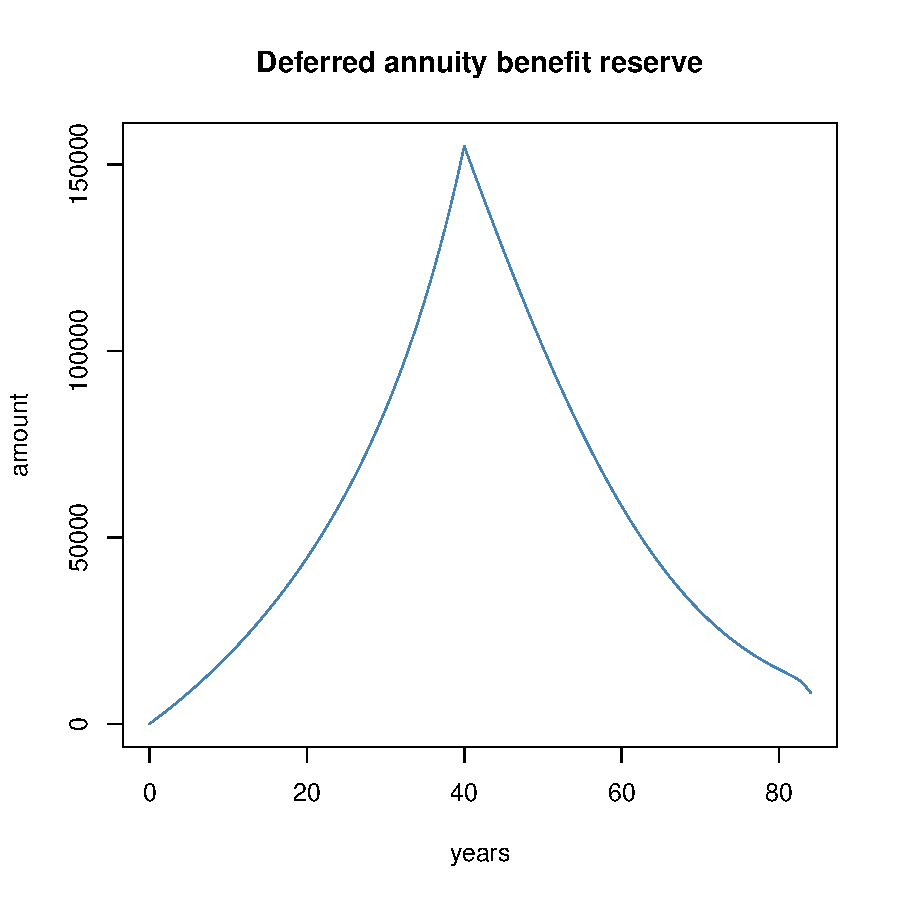
\includegraphics{an_introduction_to_lifecontingencies_package-annuityReserveGraph}
\caption{Benefit reserve profile for the exemplified annuity contract}
\label{fig:annres}
\end{center}
\end{figure}

\clearpage

\subsubsection{Expense considerations}\label{sss:expenses}

The premium paid by the policyholder usually contains an allowance for expenses
and profit loading. Expenses cover policy servicing and the producers' commissions. The insurers' profit load is explicitly  taken into account  in the  benefit premium as a flat amount, or, sometimes, as a percentage of the final premium. In other cases  implicit profit  loading is generated by using demographic and financial assumptions more prudentially than would be necessary. The equivalence principle can be extended to both the gross premium, $G$, and the expense augmented reserve,  ${}_{t}V^{E}$, when expense
allowances are taken into account by using Equation~\ref{eq:ExpenseLoad}.


\begin{equation}
\begin{gathered}
  G = \text{APV}\left(\text{Benefits}\right) + \text{APV}\left(\text{Expenses}\right) \hfill \\
 {}_{t}V^{E} = \text{APV} \left(\text{Benefits}\right) + \text{APV} \left(\text{Expenses}\right) - \text{APV} \left(\text{Gross Premium}\right)	\hfill \\ 
\end{gathered}
\label{eq:ExpenseLoad}
\end{equation}

The following example shows how an expense loaded premium $G$ is calculated for a \$ 100,000 whole life insurance on a 35 year old policyholder. 10\% of premium expense per year, 25 policy expenses per year, and annual maintenance expense of 2.5 per
1,000 units of capital are assumed.\\

The equation to be solved is $G * \ddot{a}_{35} = 100000 * A_{35} + \left( 2.5*100000/1000 + 25 + 0.1 G \right) * \ddot{a}_{35}$.
\begin{Schunk}
\begin{Sinput}
R> G <- (100000*Axn(soa08Act, x=35) + (2.5*100000/1000 + 25)*
+  			axn(soa08Act,x=35))/((1-.1)*axn(soa08Act,x=35))
R> G
\end{Sinput}
\begin{Soutput}
[1] 1234.712
\end{Soutput}
\end{Schunk}



\subsubsection{Insurances and annuities on two lives}\label{sec:ssstwoheads}

The package provides functions designed to evaluate life insurances and annuities
on two lives.
The following example checks the actuarial mathematics identity on joint and last survival status annuities 
expressed by Equation~\ref{eq:annJoinLast}.

\begin{equation}
  a_{\overline{xy}}= a_{x} + a_{y} - a_{xy}
\label{eq:annJoinLast}
\end{equation}






\begin{Schunk}
\begin{Sinput}
R> twoLifeTables <- list(maleTable=soa08Act, femaleTable=soa08Act)
R> axn(soa08Act, x=65,m=1)+axn(soa08Act, x=70,m=1)-
+  axyn(soa08Act,soa08Act,	x=65,y=70,status="joint",m=1) 
\end{Sinput}
\begin{Soutput}
[1] 10.35704
\end{Soutput}
\begin{Sinput}
R> axyzn(tablesList=twoLifeTables, x=c(65,y=70), status="last",m=1)
\end{Sinput}
\begin{Soutput}
[1] 10.35704
\end{Soutput}
\end{Schunk}

Finally, reversionary annuities (annuities payable to life y upon death of x)
APVs, $a_{x|y}=a_{y} - a_{xy}$, can also be computed by combining
\pkg{lifecontingencies} functions as the code below shows.

\begin{Schunk}
\begin{Sinput}
R> axn(actuarialtable = soa08Act, x=60,m=1)-
+  		axyzn(tablesList = twoLifeTables, 
+  				x=c(65,60),status="joint",m=1)
\end{Sinput}
\begin{Soutput}
[1] 2.695232
\end{Soutput}
\end{Schunk}


\subsection{Stochastic analysis}\label{ss:stochastic}
This last section illustrates some stochastic analysis that can be performed by the 
\pkg{lifecontingencies} package, in both demographic (
Section~\ref{sss:demo} ) and life insurance contexts (
Section~\ref{sss:actmath} ).\\

\subsubsection{Demographic examples}\label{sss:demo}

The age-until-death, both in the continuous, $\tilde T_x$,  or curtate form, $\tilde K_x$, is a stochastic variable whose 
distribution is intrinsic in the deaths within a life table.  Therefore, a
dedicated function, \code{rLife}, has been designed within
the \pkg{lifecontingencies} package to draw a sample from either  $\tilde K_x$ or $\tilde T_x$. Drawing from $K_x$ is quite simple: the distribution of the curtate future lifetime is defined as
$\Pr \left[ {{{\tilde K}_x} = t} \right] = \frac{{{d_{x + t}}}}{{\sum\limits_{j = 0}^{\omega  - x} {{l_{x + j}}} }}$, and it is passed as a
\code{prob} parameter to base \proglang{R} \code{sample} function. For example,
the code below shows how the \code{rLife} function can be used to draw a sample of
size five from the curtate future lifetime of a policyholder aged 45 as implied by
the SOA life table.

\begin{Schunk}
\begin{Sinput}
R> rLife(n = 5, object = soa08Act, x = 45, type = "Kx")
\end{Sinput}
\begin{Soutput}
[1] 18 29 12 51 35
\end{Soutput}
\end{Schunk}

\code{rLifexyz} represents the multiple lives extension of the \code{rLife}
function. It returns a matrix of sampled expected future lifetimes of $J$
policyholders given a list of $J$ lifetables. The simulation approach is
useful in evaluating demographic quantities when the analytical approach is
not feasible.
One example could be the expected years of widowhood, which
Equation~\ref{eq:widowhood} defines. $\tilde T_x$ and $\tilde T_y$ in
Equation~\ref{eq:widowhood} stand for complete future lifetimes for 
the husband and the wife respectively.

\begin{equation}
E\left[ \tilde W_y \right] = \max \left( 0, \tilde T_y - \tilde T_x \right)
\label{eq:widowhood}
\end{equation}

The following code shows how this function could be used to 
evaluate the expected years of widowhood for the wife of a couple. The
example makes use of the Italian projected life tables ips55M and ips55F, whose
derivation was shown in Section~\ref{ss:lfActT}.


\begin{Schunk}
\begin{Sinput}
R> futureLifetimes <- as.data.frame(rLifexyz(n=numSim, 
+  				tablesList=list(husband=ips55M,wife=ips55F),
+  				x=c(68,65), type="Tx"))
R> names(futureLifetimes) <- c("husband","wife")
R> temp <- futureLifetimes$wife - futureLifetimes$husband
R> futureLifetimes$widowance  <-  sapply(temp, max,0)
R> mean(futureLifetimes$widowance)
\end{Sinput}
\begin{Soutput}
[1] 7.5
\end{Soutput}
\end{Schunk}


\begin{figure}
\begin{center}
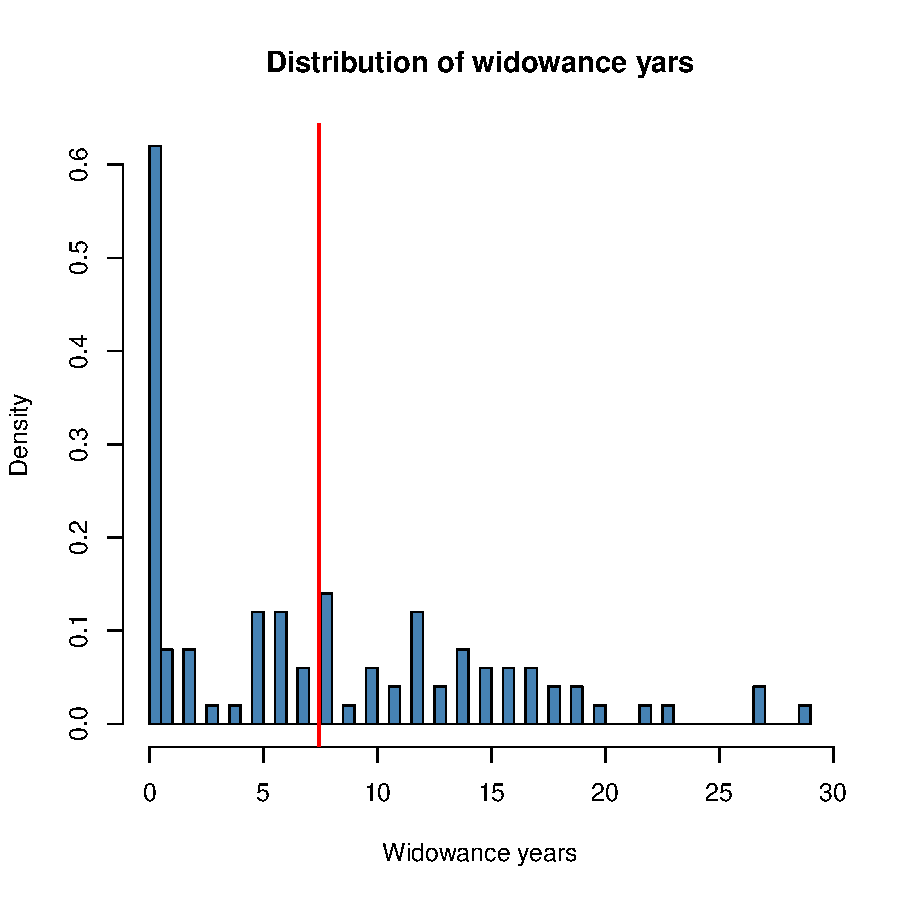
\includegraphics{an_introduction_to_lifecontingencies_package-widowanceFig}
\caption{Years of widowance distribution, where the red line represents the expected
value.}
\label{fig:widowanceFig}
\end{center}
\end{figure}

\clearpage

Finally, Figure~\ref{fig:widowanceFig} shows the distribution of widowance years 
as determined in the previous example.





\subsubsection{Actuarial mathematics examples}\label{sss:actmath}

The present value of the future benefits cash flows distribution, $\tilde Z$,
is a random variable. It is a function of both the interest rate and the 
indicator variables which are determined by the life status of the insured. Both of these quantities can be deemed stochastic. However, interest rates are considered
deterministic within the framework of the current version of \pkg{lifecontingencies} package.\\
The generation of $n$-size variates from  $\tilde Z$ is performed by the following
algorithm:
\begin{enumerate}
  \item Define a function, $PV$ that returns the present value of the life
  contingent insurance benefits, given the age at death of the policyholder, as
  $T_0$, $PV\left(T_0 \right)$.
  Within the  \pkg{lifecontingencies} package, present value functions have been
  defined for the most important life contingencies. Such functions are not
  visibly exported in the package namespace.
  \item Sample $n$ variates from $T_0$.
  \item Use $T_0$ variates as inputs for $PV\left(T_0 \right)$ to get variates
  from $\tilde Z$.
 \end{enumerate}

The code below shows the internal function \code{.faxn}, which returns the 
present value of a life contingent insurance. \code{.faxn} is
internally called by the \code{rLifeContingencies} function, as discussed below.
\code{T}, \code{y}, \code{n}, \code{i}, \code{m}, \code{k} represent the age at
death, the attained age, the term of the annuity, the interest rate, the deferring period, and
the fractional payment frequency respectively.

\begin{Code}
.faxn<-function(T,y,n, i, m, k=1)
{
	out <- numeric(1)
	K <- T-y 
		if(K<m) { 
			out <- 0 
		} else {
		  times <- seq(from=m, to=min(m+n-1/k,K),by=1/k) 
 		  out <- presentValue(cashFlows=rep(1/k, length(times)), 
          timeIds=times, interestRates=i)
		}
	return(out)
}
\end{Code}




Life contingency insurance functions return the APV, $E \left[ \tilde
Z \right]$, as a default value. The functions in Table~\ref{tab:actfun} compute APVs by using the current payment
technique. Another possible approach for evalutating APVs, even if computationally
inefficient, could be to draw a sample from the underlying $\tilde{Z}$ distribution and compute its
sample mean.\\ 

Every function in Table~\ref{tab:actfun} returns a sample of
size one if the \code{type} parameter default value, "EV" ( 
expected value), is overridden by the string "ST" ( stochastic).\\
However, when samples of greater size are required, the most straightforward 
approach is the \code{rLifeContingencies} function. The code below
shows how to generate $\tilde Z$ variates from either term life insurances, increasing
term insurances, temporary annuities, or endowment insurances respectively.
For each example, the lack of bias is verified by comparing the mean of the
sample with the theoretical APV using a classical t - test. All examples refer 
to an individual aged 20 with a 40 year insurance.
Figure~\ref{fig:Zdistrs} shows the resulting $\tilde Z$ distributions.

\begin{Schunk}
\begin{Sinput}
R> APVAxn <- Axn(soa08Act,x=25,n=40,type="EV")
R> APVAxn
\end{Sinput}
\begin{Soutput}
[1] 0.0479709
\end{Soutput}
\begin{Sinput}
R> sampleAxn <- rLifeContingencies(n=numSim, lifecontingency="Axn",
+  		object=soa08Act,x=25,t=40,parallel=FALSE)
R> tt1 <-t.test(x=sampleAxn,mu=APVAxn)$p.value
R> APVIAxn <- IAxn(soa08Act,x=25,n=40,type="EV")
R> APVIAxn
\end{Sinput}
\begin{Soutput}
[1] 1.045507
\end{Soutput}
\begin{Sinput}
R> sampleIAxn <- rLifeContingencies(n=numSim, lifecontingency="IAxn",
+  		object=soa08Act,x=25,t=40,parallel=FALSE)
R> tt2 <-t.test(x=sampleIAxn,mu=APVIAxn)$p.value
R> APVaxn <- axn(soa08Act,x=25,n=40,type="EV")
R> APVaxn
\end{Sinput}
\begin{Soutput}
[1] 15.46631
\end{Soutput}
\begin{Sinput}
R> sampleaxn <- rLifeContingencies(n=numSim, lifecontingency="axn",
+  		object=soa08Act,x=25,t=40,parallel=FALSE)
R> tt3 <- t.test(x=sampleaxn,mu=APVaxn)$p.value
R> APVAExn <- AExn(soa08Act,x=25,n=40,type="EV")
R> APVAExn
\end{Sinput}
\begin{Soutput}
[1] 0.1245488
\end{Soutput}
\begin{Sinput}
R> sampleAExn <- rLifeContingencies(n=numSim, lifecontingency="AExn",
+  		object=soa08Act,x=25,t=40,parallel=FALSE)
R> tt4 <-t.test(x=sampleAExn,mu=APVAExn)$p.value
R> c(tt1, tt2,tt3, tt4)
\end{Sinput}
\begin{Soutput}
[1] 0.07716977 0.61236632 0.85234323 0.81753278
\end{Soutput}
\end{Schunk}


\begin{figure}
\begin{center}
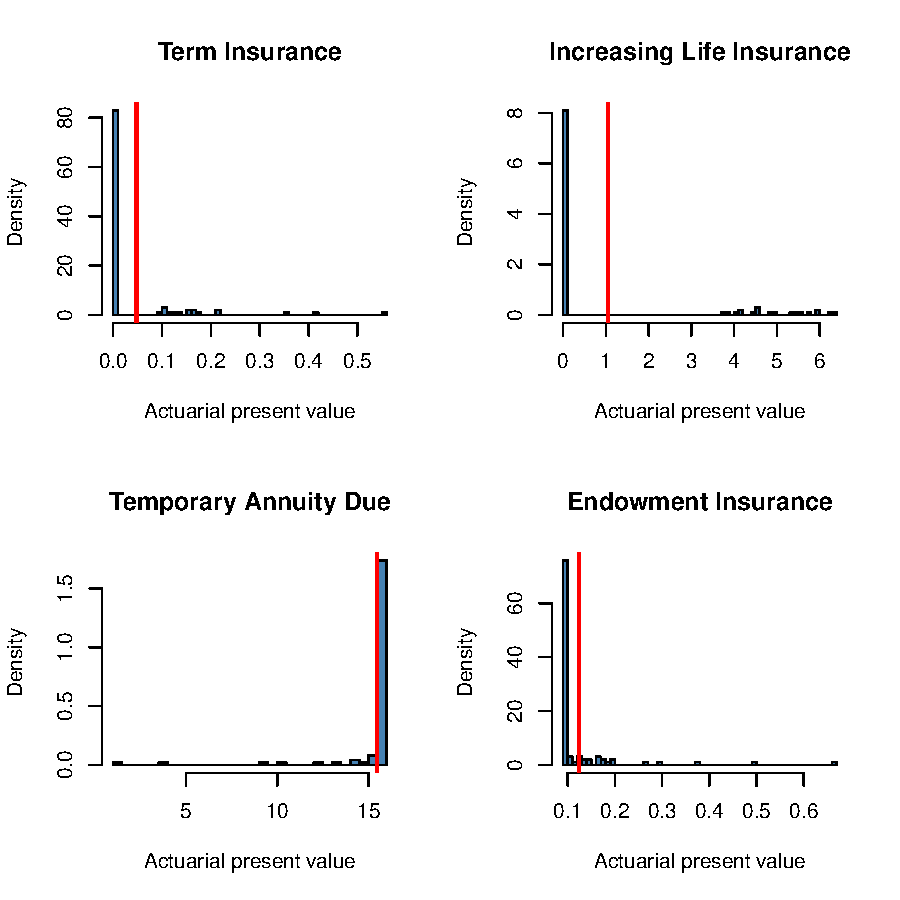
\includegraphics{an_introduction_to_lifecontingencies_package-figsim}
\caption{Life insurance stochastic variables distributions. Red vertical line represents APV.}
\label{fig:Zdistrs}
\end{center}
\end{figure}

The same analysis can be performen on life contingencies insurance on two (or more lives)
as listings exemplify below.

\begin{Schunk}
\begin{Sinput}
R> tablesList=list(soa08Act,soa08Act);x=c(60,60);m=0;status="first";t=30;k=1
R> APVAxyz<-Axyzn(tablesList=tablesList,x=x,n=t,status=status,type="EV")
R> samplesAxyz<-rLifeContingenciesXyz(n=numSim,lifecontingency = "Axyz",
+  		tablesList = tablesList,x=x,t=t,m=m,k=k,status=status,
+  		parallel=FALSE)
R> tt5<-t.test(x=samplesAxyz, mu=APVAxyz)$p.value
R> APVaxyz<-axyzn(tablesList=tablesList,x=x,n=t,m=m,k=k,status=status,type="EV")
R> samplesaxyz<-rLifeContingenciesXyz(n=numSim,lifecontingency = "axyz",
+  		tablesList = tablesList,x=x,t=t,m=m,k=k,status=status,
+  		parallel=FALSE)
R> tt6<-t.test(x=samplesaxyz, mu=APVaxyz)$p.value
R> c(tt5,tt6)
\end{Sinput}
\begin{Soutput}
[1] 0.2606326 0.4692603
\end{Soutput}
\end{Schunk}



All contingency functions have been provided an argument \code{power}, whose
default value is set to one, that becomes useful when moments higher than one
(the expected) of the life contingency random variable are needed. For example a
direct computation of term insurance variance can be performed as follows.

\begin{Schunk}
\begin{Sinput}
R> var(sampleAxn)
\end{Sinput}
\begin{Soutput}
[1] 0.008045913
\end{Soutput}
\begin{Sinput}
R> Axn(soa08Act, x=25,n=40, power=2)-Axn(soa08Act, x=25,n=40, power=1)^2
\end{Sinput}
\begin{Soutput}
[1] 0.01468878
\end{Soutput}
\end{Schunk}

The example that follows verifies that the variance an endowment insurance, 
calculated by the rule of moments, matches with the variance of the simulated
distribution.


The full distribution of a life contingent insurance variable $\tilde Z$, can be
used to compute premiums using the percentile premium principle. Under this
approach, the premium is set to ensure that the insurer will suffer financial loss
with a sufficiently low probability (made explicit by the percentile).\\
An example will clarify the concept. For a 40 - year
insurance on a single policyholder aged 25, the actuarial present value of benefits, 
i.e., the expected value of discounted future benefits, would be

\begin{Schunk}
\begin{Sinput}
R> APV <- Axn(actuarialtable = soa08Act, x=25, n=40)
R> APV
\end{Sinput}
\begin{Soutput}
[1] 0.0479709
\end{Soutput}
\end{Schunk}

while the benefit premium at the 90th percentile, that is, the premium that would
make the insurer incurr an underwriting loss with 10\% probability,
would be




\begin{Schunk}
\begin{Sinput}
R> samples <- rLifeContingencies(n=numSim, lifecontingency = "Axn", 
+  		object= soa08Act, x=25,t=40,parallel=FALSE)
R> pct90Pr <- as.numeric(quantile(samples,.90))
R> pct90Pr
\end{Sinput}
\begin{Soutput}
[1] 0.1234772
\end{Soutput}
\end{Schunk}

Finally, if $N=1000$ similar policyholders were insured, the Law of Large
Numbers would lead to a strong reduction in the premium charged on each
policyholder, as computed below.

\begin{Schunk}
\begin{Sinput}
R> pct90Pr2 <- qnorm(p=0.90,mean=APV, sd=sd(samples)/sqrt(1000))
R> pct90Pr2
\end{Sinput}
\begin{Soutput}
[1] 0.05307157
\end{Soutput}
\end{Schunk}


The final example in this paper shows how the stochastic functions bundled in
the \pkg{lifecontingencies} package can be used to make an actuarial appraisal of embedded benefits.\\
Suppose a corporation grants its 100 employees life insurance benefits equal to
their annual salary and payable at the month of death. Moreover, suppose that:
\begin{enumerate}
	\item The expected value and the standard deviation of the salary are \$ 50,000 and \$ 15,000 respectively and the 
	salaries follow a log-normal distribution.
	\item The distribution of the employees' age  is uniform on [25,65]. Assume 65 is the retirement age.
	\item The SOA illustrative table represents an unbiased description of the
	population mortality.
	\item Assume no lapse to hold.
	\item The policy length is annual.
\end{enumerate}

We evaluated the best estimate, or the fair value of the insured benefits according 
to both IFRS accounting standards and risk
margin measure. In this example, the risk margin measure, which is the difference between the 75th percentile and the best estimate, will be used. IFRS
standards \citep{ifrsInsurance} define the fair value of an insurance liability as the sum of its best estimate and its risk margin.\\

In the initial part of the example, we set up the parameter of the model and configured the parallel computation facility available with the package \pkg{parallel}. The code parallelization has been adapted from examples found in the \citep{mccallum2011parallel} textbook.

\begin{Schunk}
\begin{Sinput}
R> nsim <- 50
R> employees <- 100
R> salaryDistribution <- rlnorm(n=employees,m=10.77668944,s=0.086177696)
R> ageDistribution <- round(runif(n=employees,min=25, max=65))
R> policyLength <- sapply(65-ageDistribution, min, 1)
R> getEmployeeBenefit<-function(index,type="EV") {
+  	out <- numeric(1)
+  	out <- salaryDistribution[index]*Axn(actuarialtable=soa08Act, 
+  			x=ageDistribution[index],n=policyLength[index], 
+  			i=0.02,m=0,k=1, type=type)
+  	return(out)
+  }
R> require(parallel)
R> cl <- makeCluster(1) 
R> worker.init <- function(packages) {
+  	for (p in packages) {
+  		library(p, character.only=TRUE)
+  	}
+  	invisible(NULL)
+  }
R> clusterCall(cl, 
+  		worker.init, c('lifecontingencies'))
\end{Sinput}
\begin{Soutput}
[[1]]
NULL
\end{Soutput}
\begin{Sinput}
R> clusterExport(cl, varlist=c("employees","getEmployeeBenefit",
+  				"salaryDistribution","policyLength",
+  				"ageDistribution","soa08Act"))
\end{Sinput}
\end{Schunk}
Then we perform best estimate and risk margin calculations.

\begin{Schunk}
\begin{Sinput}
R> employeeBenefits <- numeric(employees)
R> employeeBenefits <- parSapply(cl, 1:employees,getEmployeeBenefit, type="EV")
R> employeeBenefit <- sum(employeeBenefits)
R> benefitDistribution<-numeric(nsim)
R> yearlyBenefitSimulate<-function(i)
+  {
+  	out <- numeric(1)
+  	expenseSimulation <- numeric(employees)
+  	expenseSimulation <- sapply(1:employees, getEmployeeBenefit, type="ST")
+  	out <- sum(expenseSimulation)
+  	return(out)
+  }
R> benefitDistribution <- parSapply(cl, 1:nsim,yearlyBenefitSimulate )
R> stopCluster(cl)
R> riskMargin <- as.numeric(quantile(benefitDistribution,.75)-employeeBenefit)
R> totalBookedCost <- employeeBenefit+riskMargin
R> employeeBenefit
\end{Sinput}
\begin{Soutput}
[1] 22370.38
\end{Soutput}
\begin{Sinput}
R> riskMargin
\end{Sinput}
\begin{Soutput}
[1] 26195.4
\end{Soutput}
\begin{Sinput}
R> totalBookedCost
\end{Sinput}
\begin{Soutput}
[1] 48565.78
\end{Soutput}
\end{Schunk}


\section{Discussion}\label{sec:discussion}
\subsection{Advantages, limitations, and future perspectives}

The \pkg{lifecontingencies} package allows actuaries to perform
demographic, financial and actuarial mathematics calculations within
\proglang{R}; in particular, life contingent insurance contracts can
be priced and reserved. In addition, a peculiar feature of
\pkg{lifecontingencies} is its ability to generate variates from the
future life time and the underlying stochastic distributions of life
contingent insurances.

One of the most significant limitations of the most recent
(version~1.0) \pkg{lifecontingenciess} package release is that only
single decrements tables can be handled.  In addition, continuous-time
life contingent models are currently not handled explicitly.

We expect to remove such limitations in the future. In addition, we
expect to provide coerce methods for packages that specialize in
demographic analysis, like \pkg{demography} and
\pkg{LifeTables}. Furthermore, we wish to allow easier sharing of
analyses with interest rate modeling packages like \pkg{termstrc}.

Finally, code optimization and improvement is carried out
continuously. The extension of parallel computation features, memory
usage profiling, and the use of \proglang{C} or \proglang{C++} code
fragments in select parts of the code have begun (for \pkg{Rcpp} package, \cite{RcppR} usage) or being 
planned for the near future.

\subsection{Accuracy}\label{sec:disclaimer}

The accuracy of the calculations has been verified by checking
numerical examples reported in \cite{bowers1997actuarial} and in the
lecture notes of "Actuarial Mathematics" taken by the author years
ago at The Catholic University of Milan \citep{mazzoleni2000appunti}. Such test have been implemented with unit root testing in the package \pkg{testthat}, \cite{pkg:testthat}.
The numerical results are identical to those reported in the cited
references for most functions, with the exception of fractional
payment annuities; for these, the answer is only reported up to the
fifth decimal. The reason for such inaccuracy is that the package
calculates the APV using the direct sum of fractional survival
probabilities, while the results reported in the cited references are
obtained by closed formulas.

Finally, it is worth noting that the package and functions herein are
provided as is without any guarantee regarding the accuracy of
calculations. The author disclaims any liability arising from
potential losses due to direct or indirect use of this package.


\section*{Acknowledgments}\label{sec:acknowledgments}

The author wishes to thank all those whose suggestions contributed to
the package's enhancements. In particular, he would like to thank
Christophe Dutang, Tim Riffle, Reinhold Kainhofer and Kevin J. Owens for their
suggestions on code and vignettes. A special thank also to Anton Sylchenko for the
copy-editing. Also, many thanks go out to the anonymous Journal of
Statistical Software referees that helped improve the quality of the
package and underlying vignettes.

%\bibliographystyle{jss}
\bibliography{lifecontingenciesBiblio}

\end{document}
